\documentclass{article}
\usepackage{graphicx} % Required for inserting images

\title{CS184 Project 2}
\author{Michael Huang}
\date{February 2024}

\begin{document}

\maketitle
In this project, we worked with both Bezier Curves and Surfaces. We investigated how Bezier Curves can be implemented through De Castelijau's algorithm, and how we can extend that to the 3d case. 
\\
\\
In the second part, we worked with 3d triangle meshes, specifically, how to traverses triangles meshes and how to preform operations on triangle meshes. We preform Edge Splits, Edge Flips, Area Normalization, and Loop Subdivision using the halfedge data structure.
\section{Bezier Curves and Surfaces}
\subsection{Bezier Curves with 1D De Casteljau Subdivision}
De  Casteljau's algorithm uses a recursive algorithm to find the point on the bezier curve. Given we have $n$ control points, we do:
$$p_i' = lerp(p_i, p_{i + 1}, t) = (1 - t)p_i + tp_{i + 1}$$
We continue this recursive step until there's only 1 point. To get the full bezier curve, we move $t \in [0, 1]$. Below is an example of an output with 6 control points. 
\begin{center}
    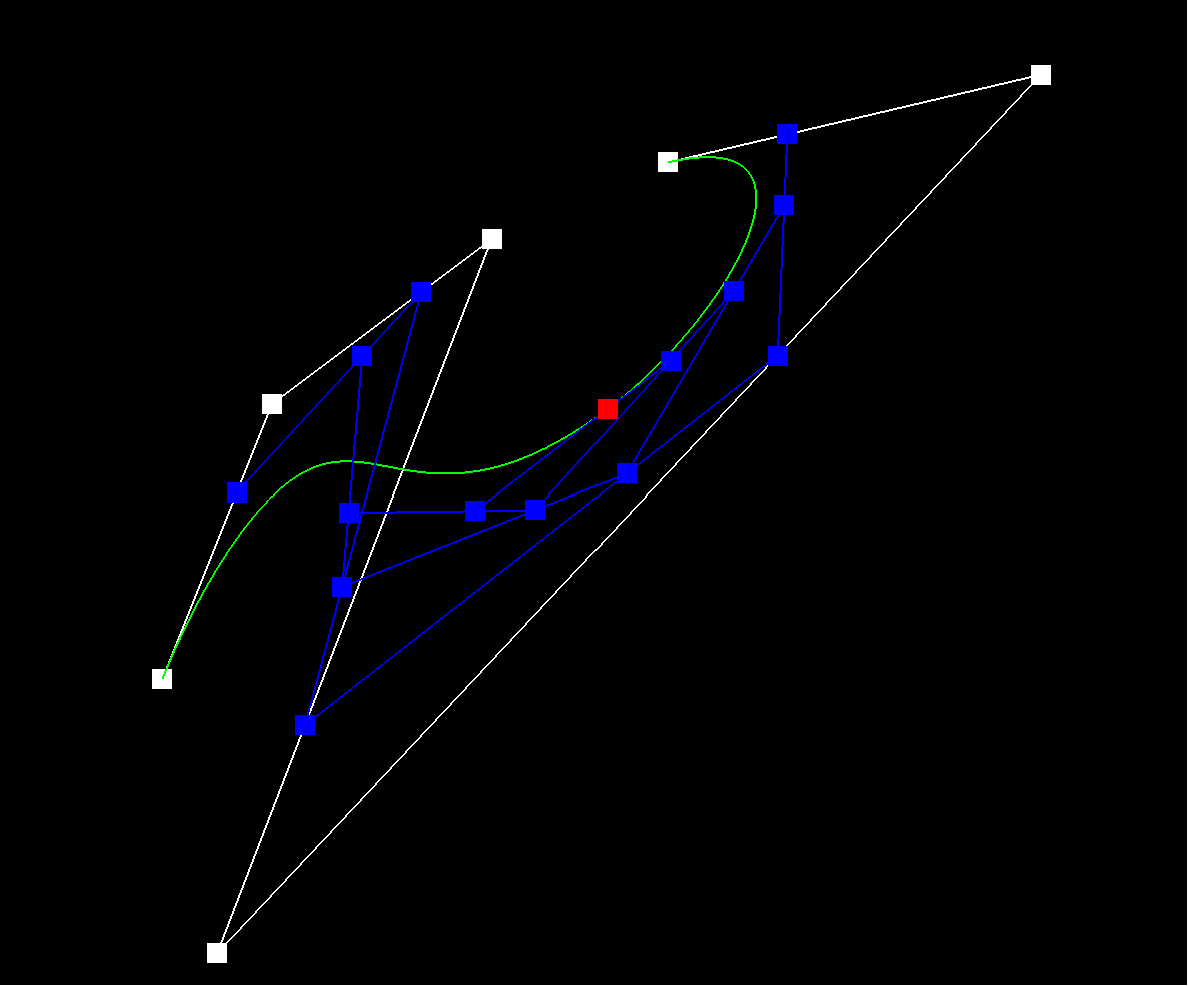
\includegraphics[]{Part 1/bez1.png}
\end{center}
To show the recursive nature of the algorithm, below is each step of De Casteljau's algorithm.
\begin{center}
    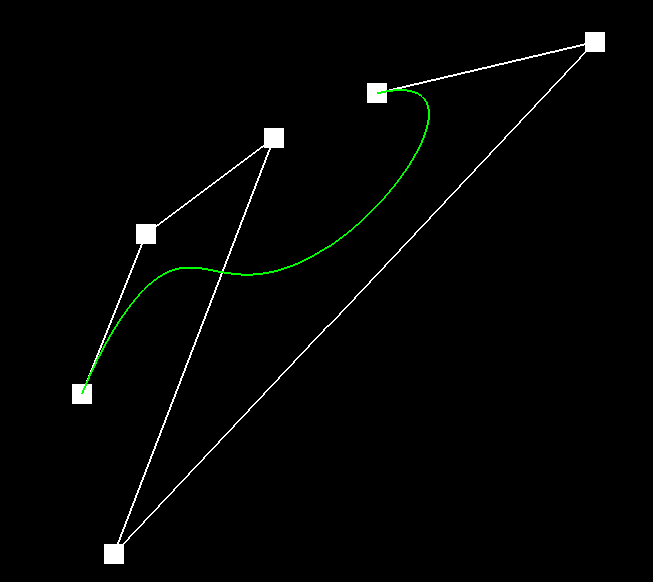
\includegraphics[]{Part 1/step1.png}
    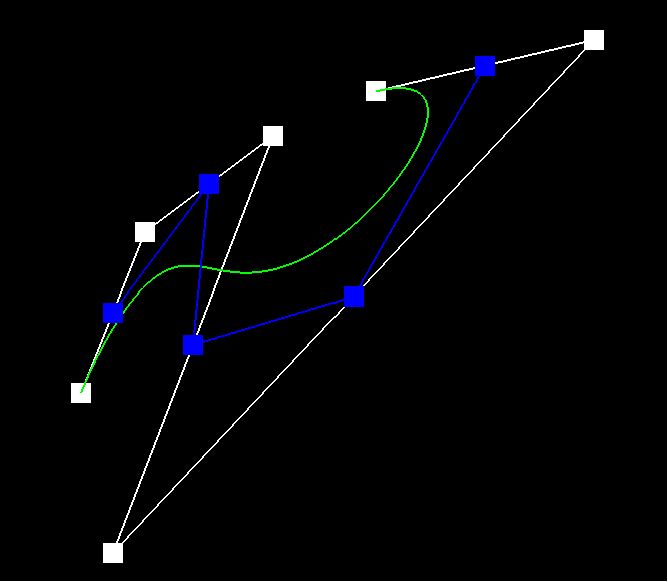
\includegraphics[]{Part 1/step2.png}
    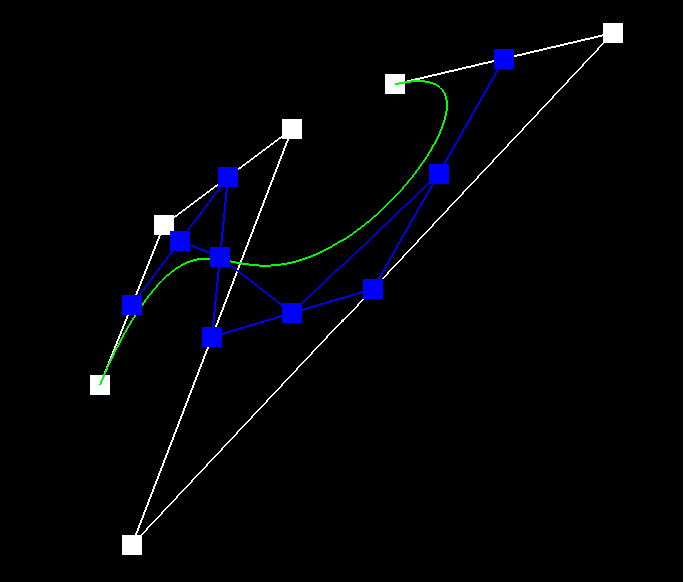
\includegraphics[]{Part 1/step3.png}
    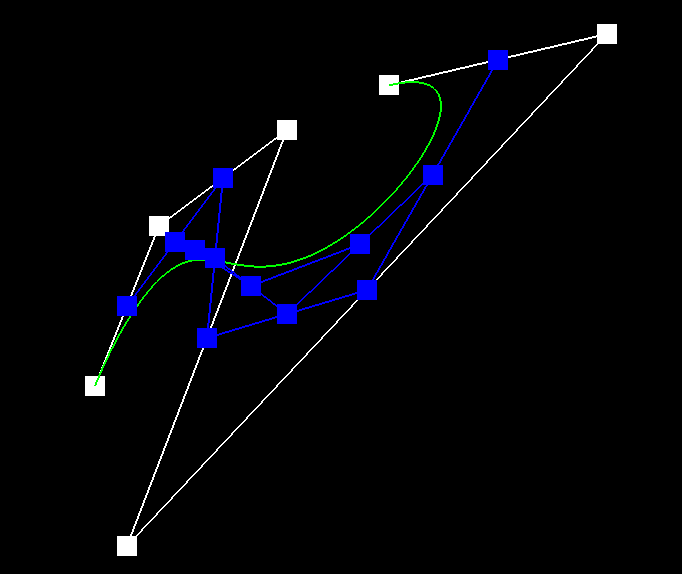
\includegraphics[]{Part 1/step4.png}
    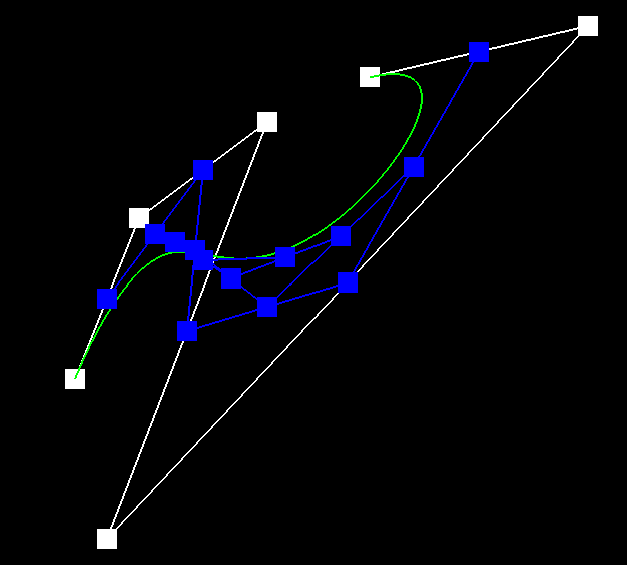
\includegraphics[]{Part 1/step5.png}
    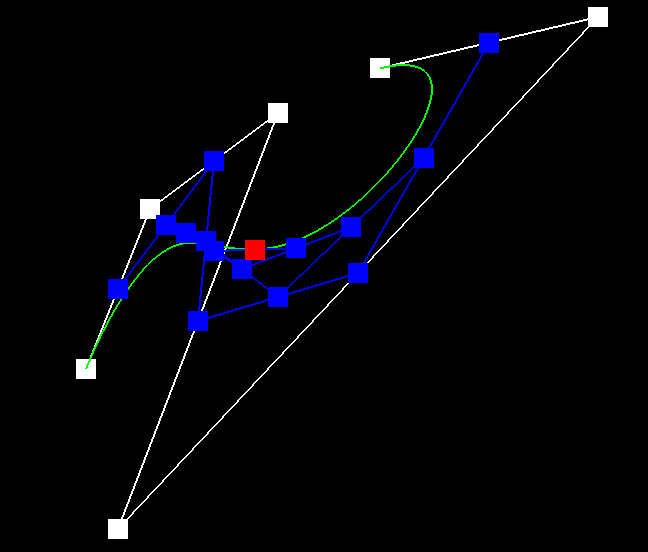
\includegraphics[]{Part 1/step6.png}
\end{center}
We can also change the location of the control point to change the curve:
\begin{center}
    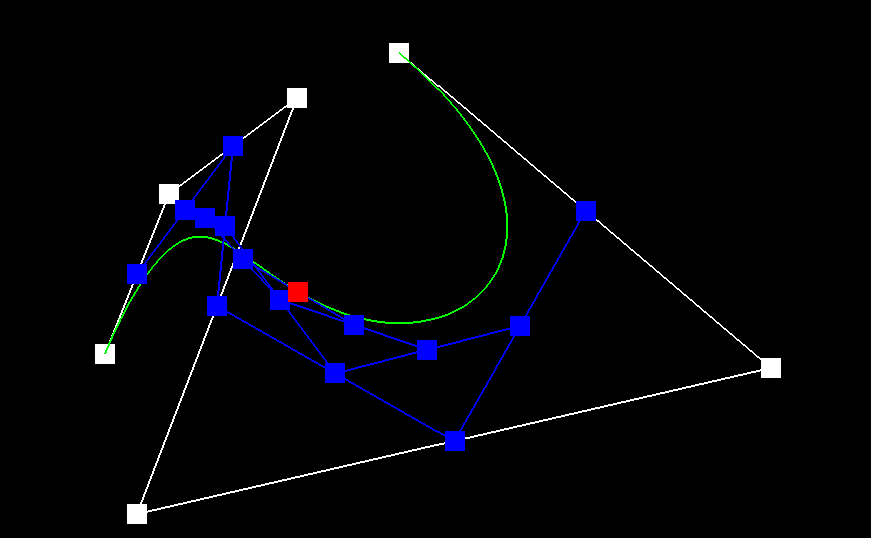
\includegraphics[]{Part 1/changed.png}
\end{center}
\subsection{Bezier Surfaces with Separable 1D de Casteljau}
We can extend toward surfaces by using $N x N$ control points. first, we create the Bezier curves for points $(P_{i, j})_{j = 1}^N\forall i \in [1, N]$. After we have the Bezier curves for some $t$, we can create the second axis Bezier curve using a seperate $u \in [0, 1]$ with the points $(P_1', P_2',...,P_N')$. This allows us to create a Bezier Surface. Below is an example using a Bezier Surface:
\begin{center}
    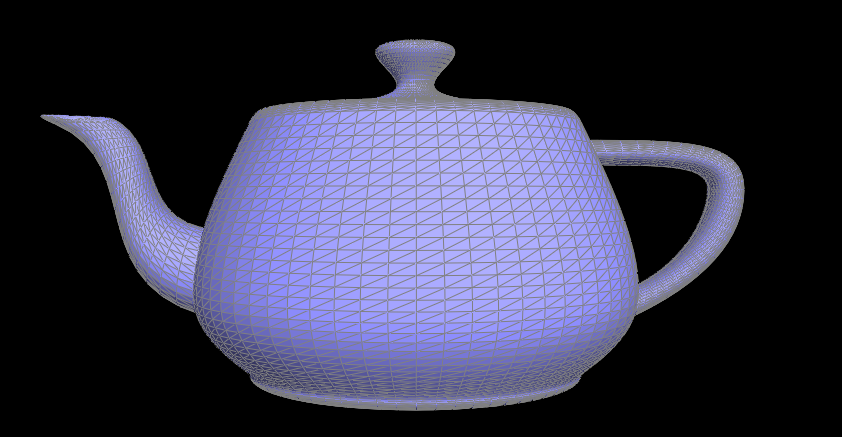
\includegraphics[scale = 0.5]{Part 2/teapot.png}
\end{center}
\section{Triangle Meshes and Half-Edge Data Structure}
\subsection{Area Weighted Vertex Normal}
We can use the Area Weighted Vertex Normal to do Phong shading. to do this, we get the area of each incident face, and taked a weighted average of the normal vectors of each face using the areas as weights. Iterating through each Normal is simple, but calculating the area of each triangle is somewhat difficult. To do this, consider vertices $A, B, C$ of each triangle. We can use $A$ as the origin, and calculate the orthogonal vector as the cross product of the two vectors $(B - A) X (C - A)$. The magnitude of the orthogonal vector will be 2x the area of the triangle, so the area of the triangle will be half the cross product. Below is the result of executing the algorithm:
\begin{center}
    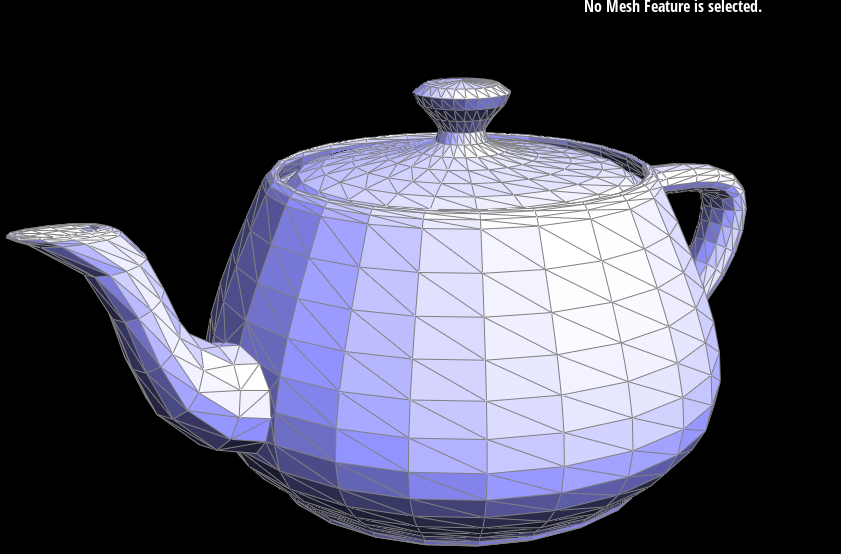
\includegraphics[]{Part 3/nophong.png}
    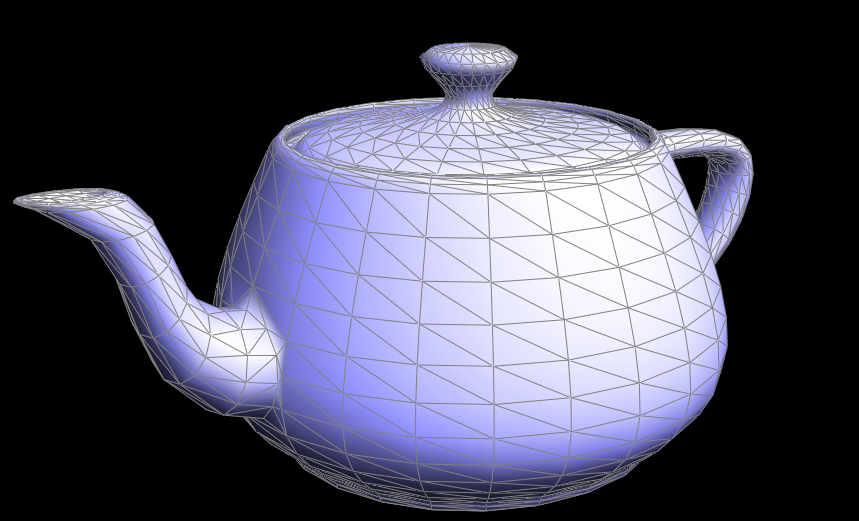
\includegraphics[]{Part 3/phong.png}
\end{center}
\subsection{Edge Flip}
To implement the edge flip, I started with the mesh from spec, with vertices $(a, b, c, d)$. Next, I used the original edge $(c, b)$ and changed the root vertex and the twin root vertex. Next, I cycled starting with (a, d), and set each pointer of each half edge in the cycle. I.e I did (a,d)->(d, c)->(c,a) and set each attribute of the halfedges. I did the same thing for the twin cycle, going (d,a)->(a,b)->(b,d). Below is an example of edge flips:
\begin{center}
    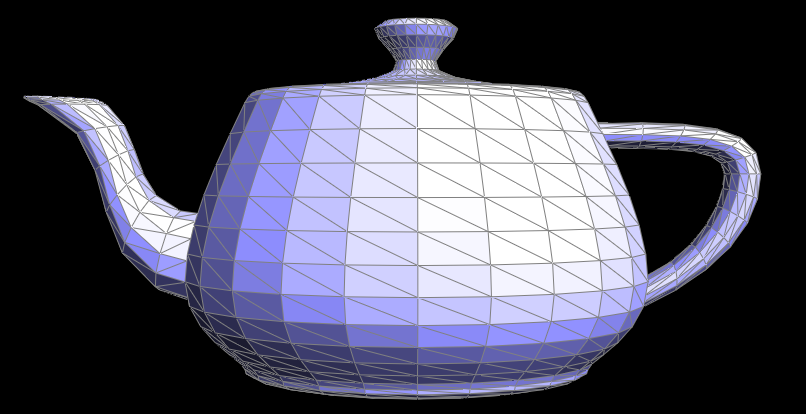
\includegraphics[]{Part 4/before.png}
    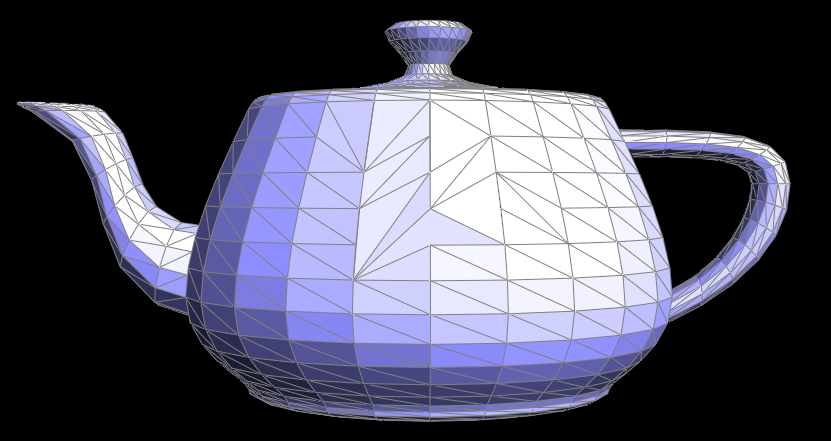
\includegraphics[]{Part 4/edgeflips.png}
\end{center}
In terms of debugging, I thought this was relatively straightforward, especially with the tips that were given. Things that helped me code was that I drew diagrams to help me.
\subsection{Edge Split}
Edge splitting was much more complex than edge flipping due to the amount of pointers. Again, I listed all pointers, but I had to create new edges, new faces, and new halfedges. Similar to edge flipping, I went through every cycle that was created from the edge splits, including the new elements, and set every attribute. There were 4 new cyles, so I just went through each cycle and set its attributes. Below is an example of a few edge splits:
\begin{center}
    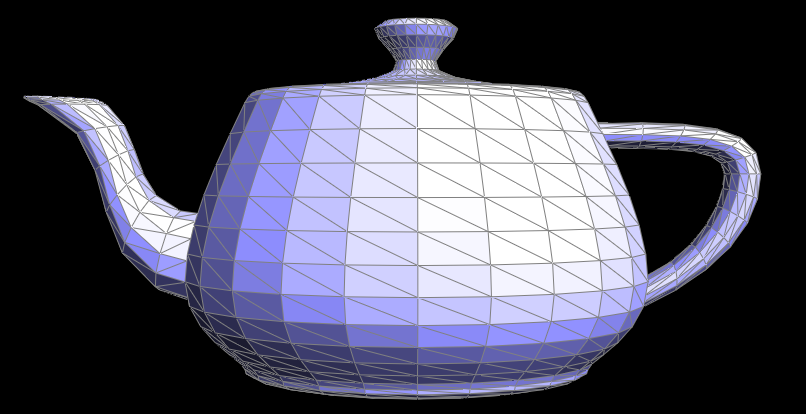
\includegraphics[]{Part 4/before.png}
    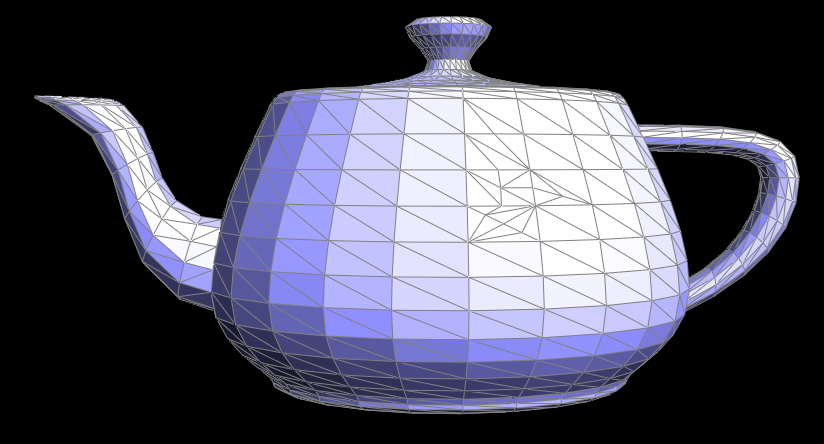
\includegraphics[]{Part 5/edgesplits.png}

\end{center}
And below is a combination of both flips and splits:
\begin{center}
    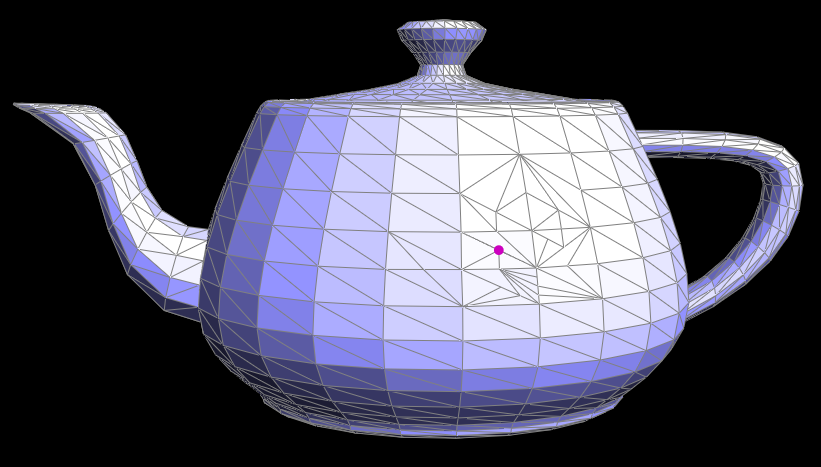
\includegraphics[]{Part 5/flipsysplits.png}
\end{center}
In terms of debugging, I thought this was relatively straightforward, especially with the tips that were given. Things that helped me code was that I drew diagrams to help me.
\\
\\
I did not implement boundary conditions for edge splits.
\subsection{Loop Subdivision For Mesh Upsampling}
To implement mesh upsampling, I would go through the following steps:
\begin{enumerate}
    \item Iterate through all original vertices $v$ in the mesh, and calculate its new position. Let $d = deg(v)$, and we set $u = 3/16$ if the degree is 3, and $u = 3/8d$ otherwise. We set the new position to be:
    $$newpos(v) = (1 - du)pos(v) + u\sum_{w 
    \in neighbors(v)} pos(v)$$

    \item Iterate through all edges in the mesh, and store the new position of the created midpoint vertex when splitting the edge. This is calculated as:
    $$newpos(m) = \frac{3}{8}(A + B) + \frac{1}{8}(C + D)$$
    Where $AB$ is the edge we split, and $C$ and $D$ are the positions of the incident vertices of $A$ and $B$. We store this new position in the edge because when we split the edge and create new vertex $m$, we can directly set the new position of $m$ to be the new position of the splitted edge.

    \item split all original edges of the mesh. To keep track of which edges have already been split, I created an attribute isSplitted to check whether an edge has been split or not. I also keep track of each edges that were original inside a variable isNew.

    \item Flip all edges that are new and connect a old vertex to a new vertex.

    \item Set all vertex positions to the new position.
\end{enumerate}
One of the tips I have is to interpret your output visually to something that can happen in your code. For example, one of the bugs I had was that when I upsampled, all of the faces would sharply move inward. I didn't really think anything of it, and thought it was a problem with my flip or split. However, if I interpretted it visually, I would understand that the vertex position is being set to 0 somewhere, leading me to believe it's something to do with position setting, which only happens in task 6. Look at it visually to figure out where the bug is!
\\
Lets take a look at an example output: the icosahedron:
\begin{center}
    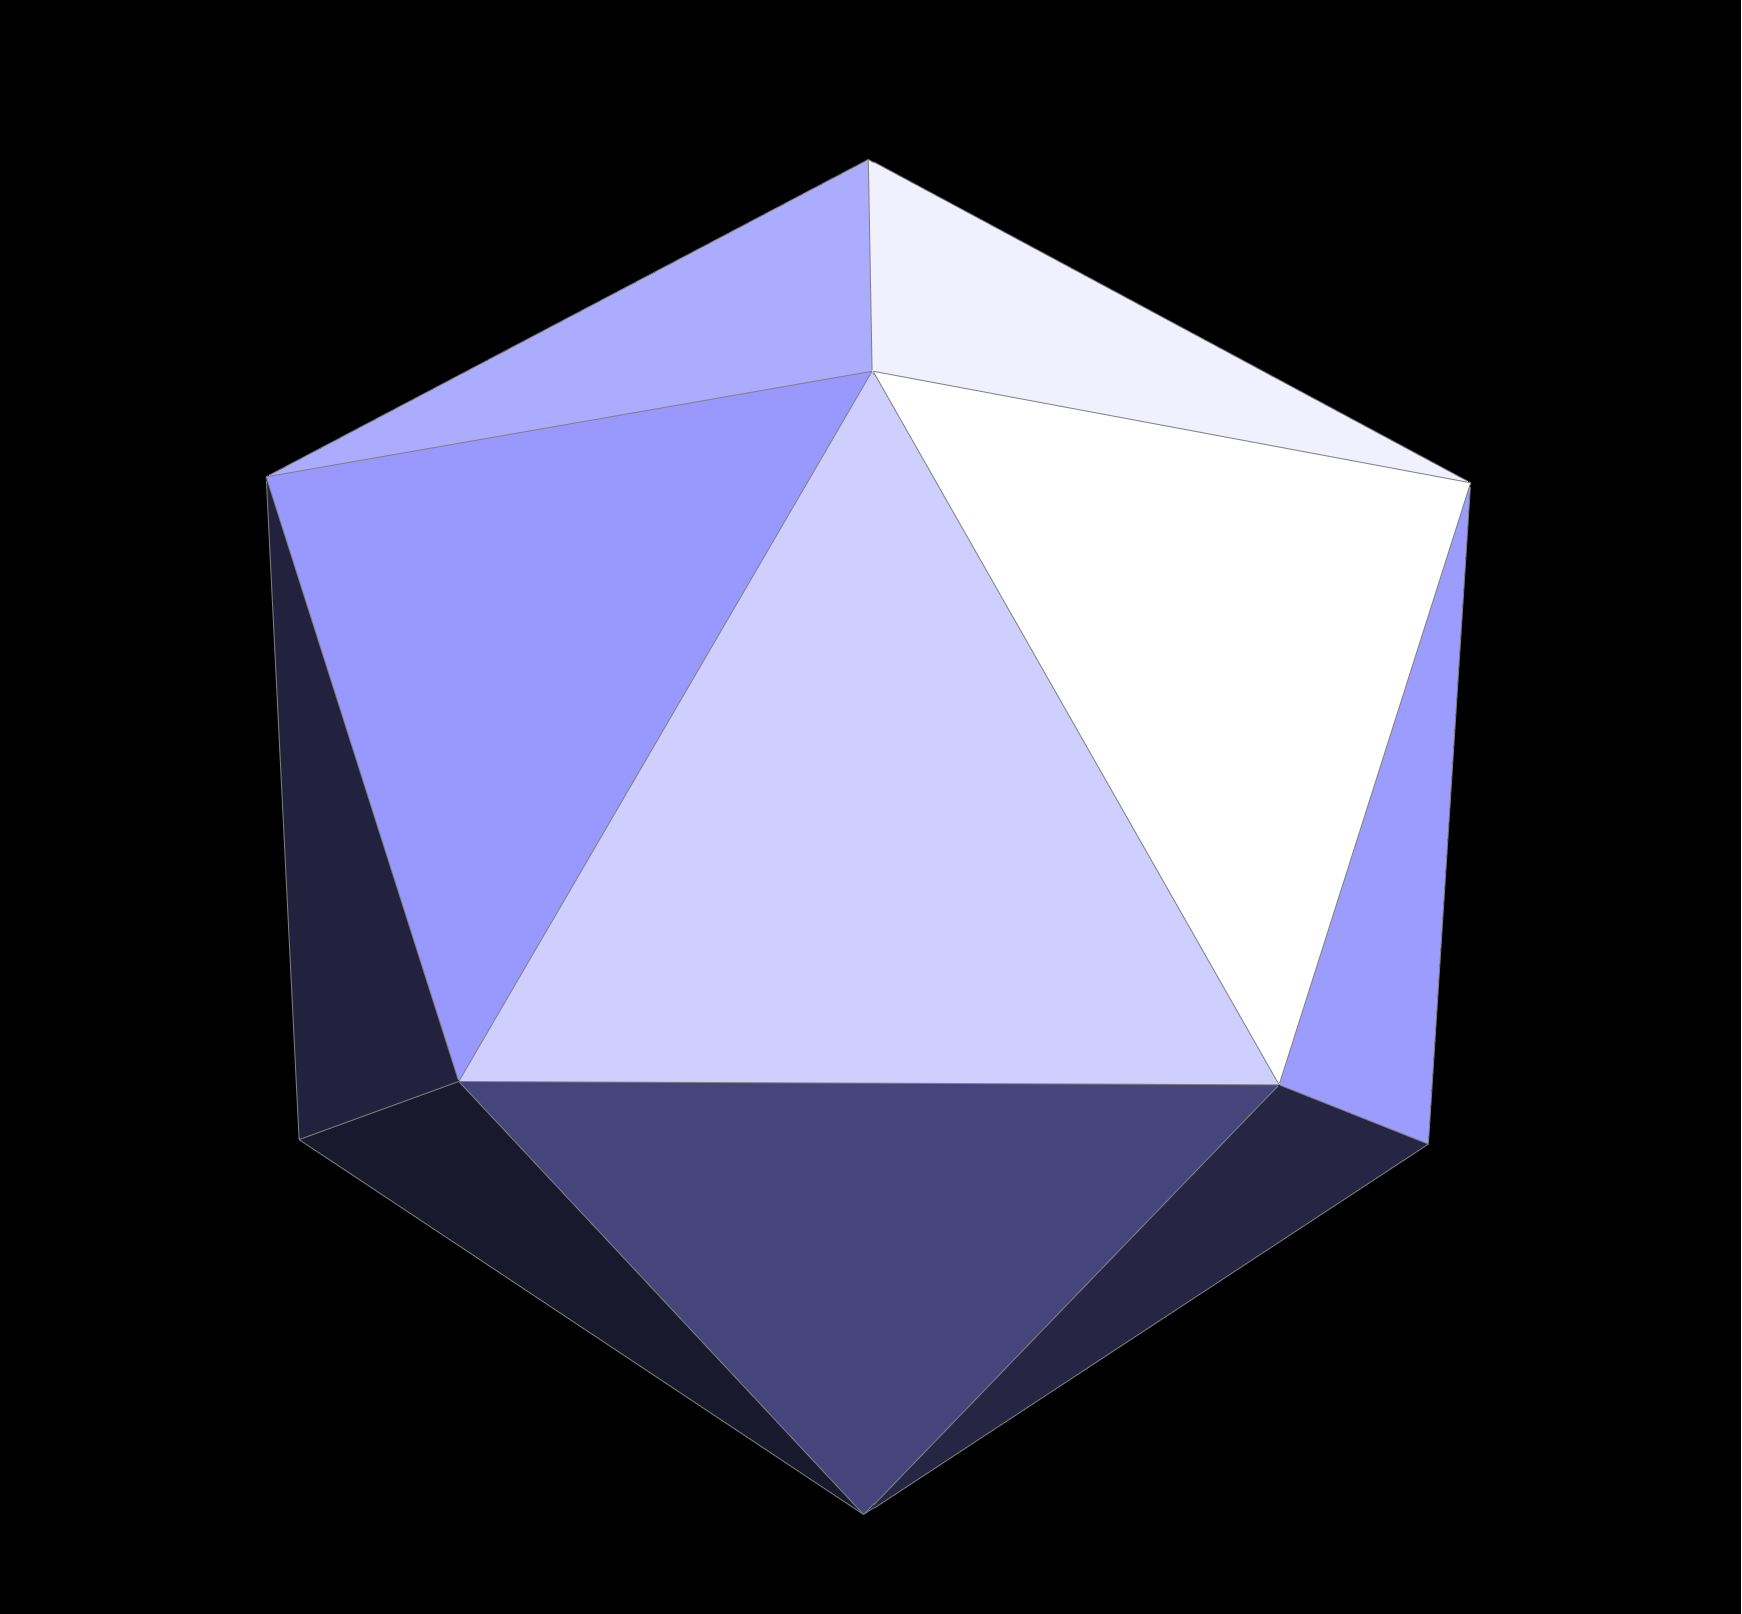
\includegraphics[]{task 6/iso1.png}
    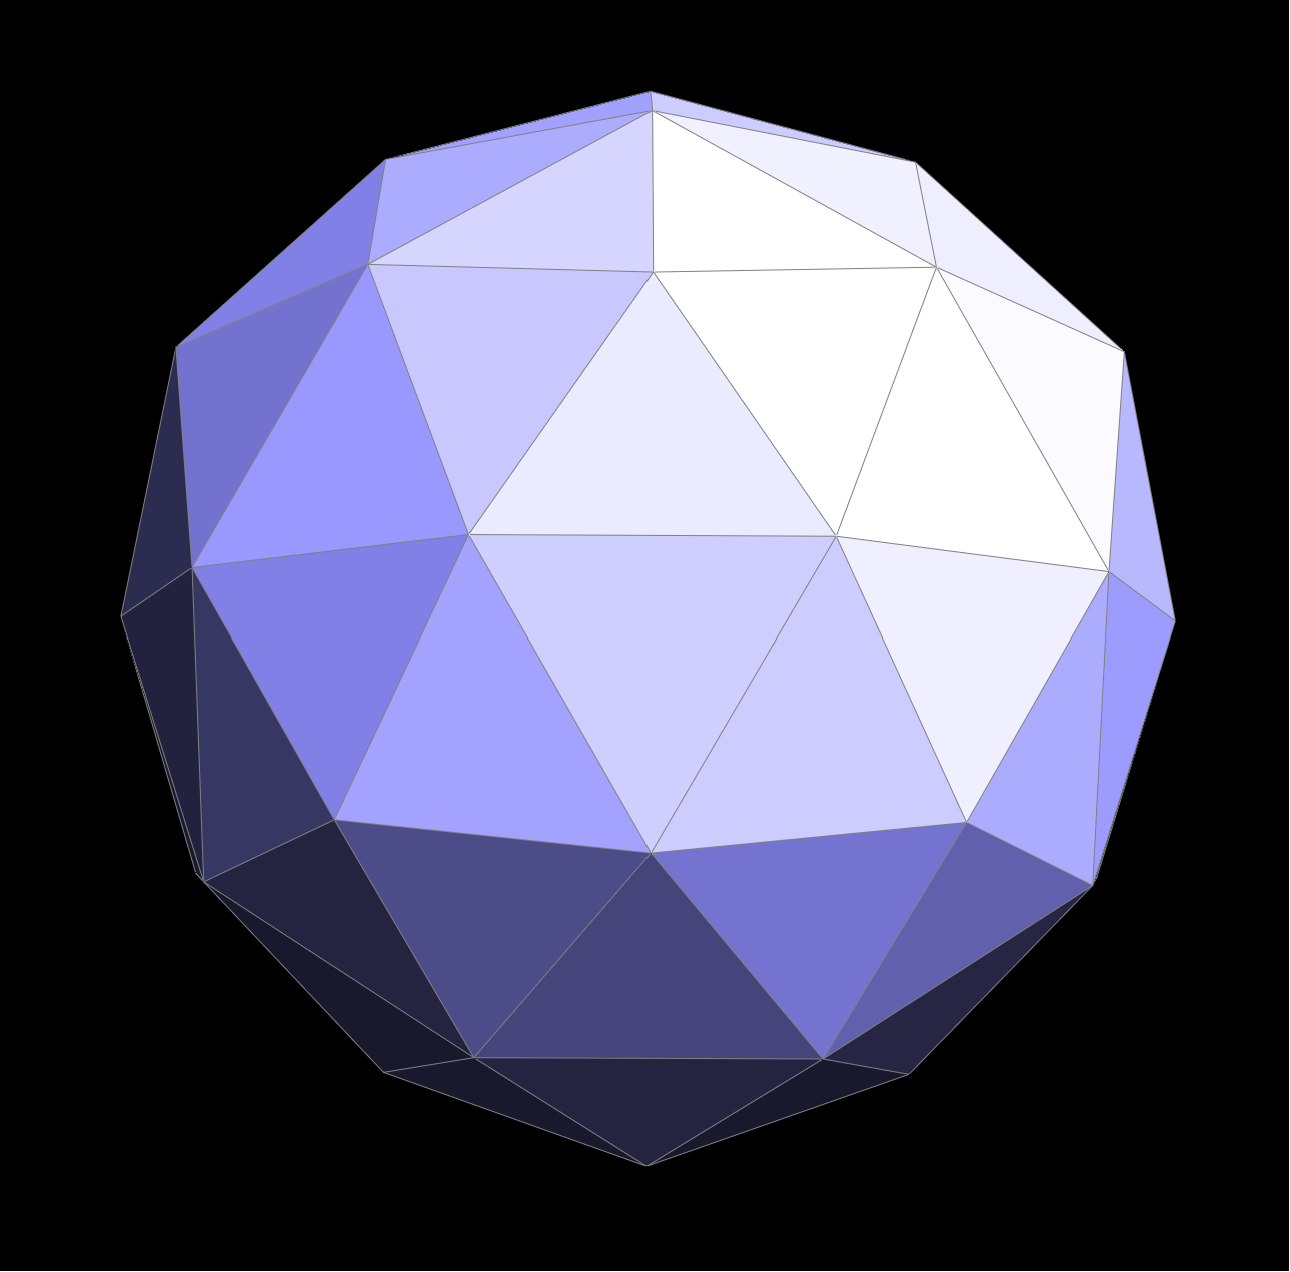
\includegraphics[]{task 6/iso2.png}
    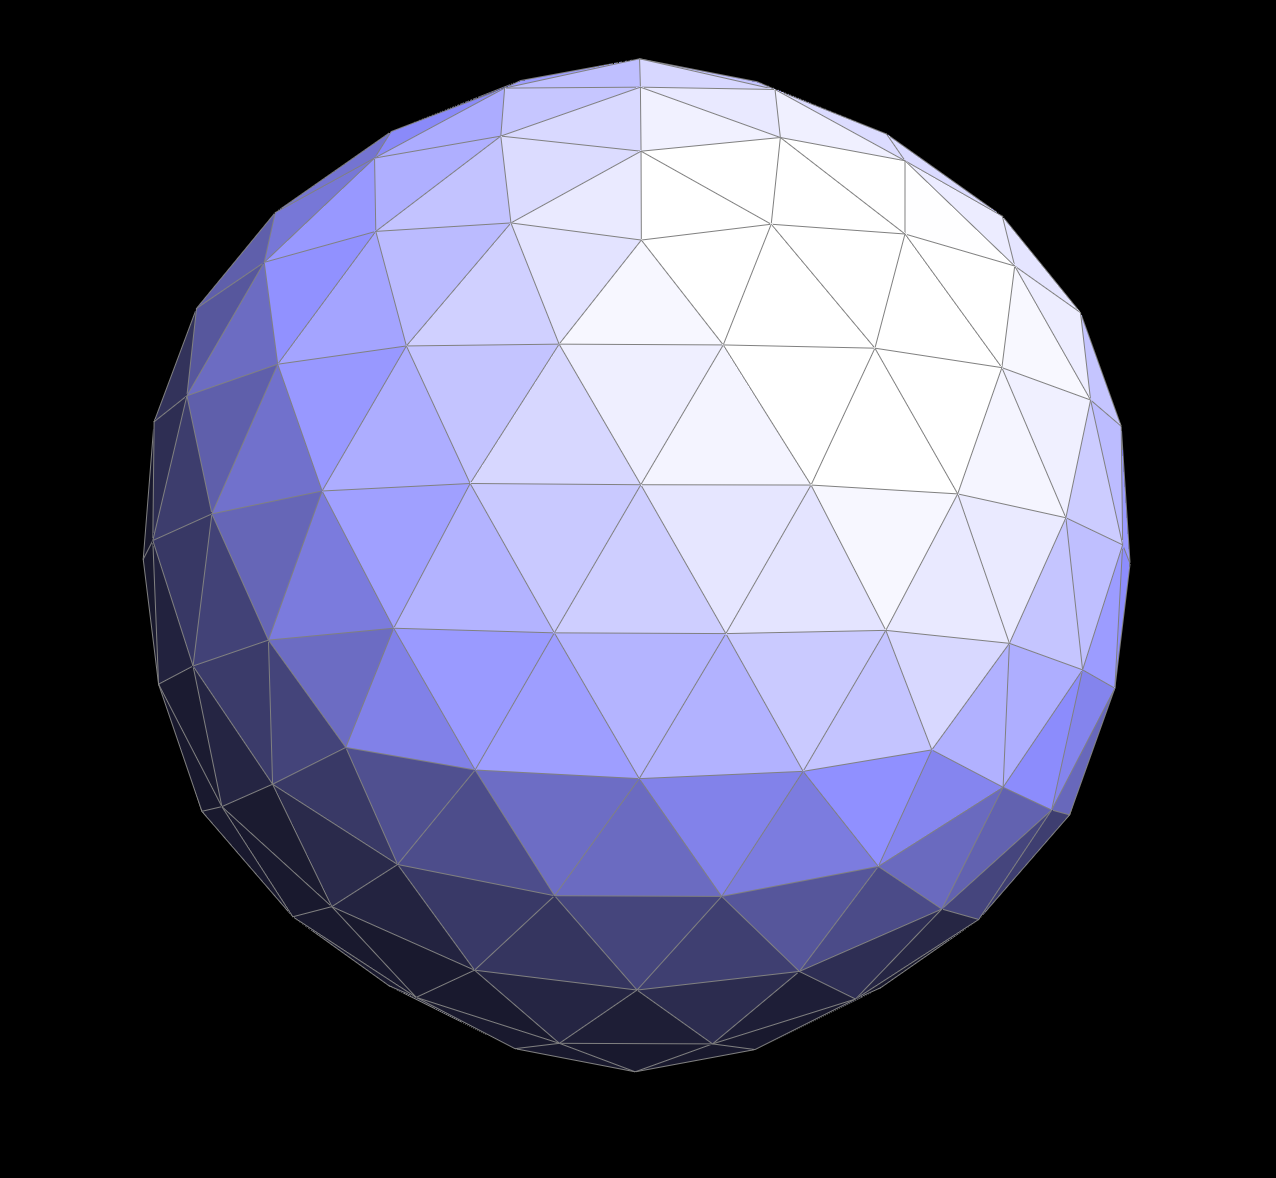
\includegraphics[]{task 6/iso3.png}
    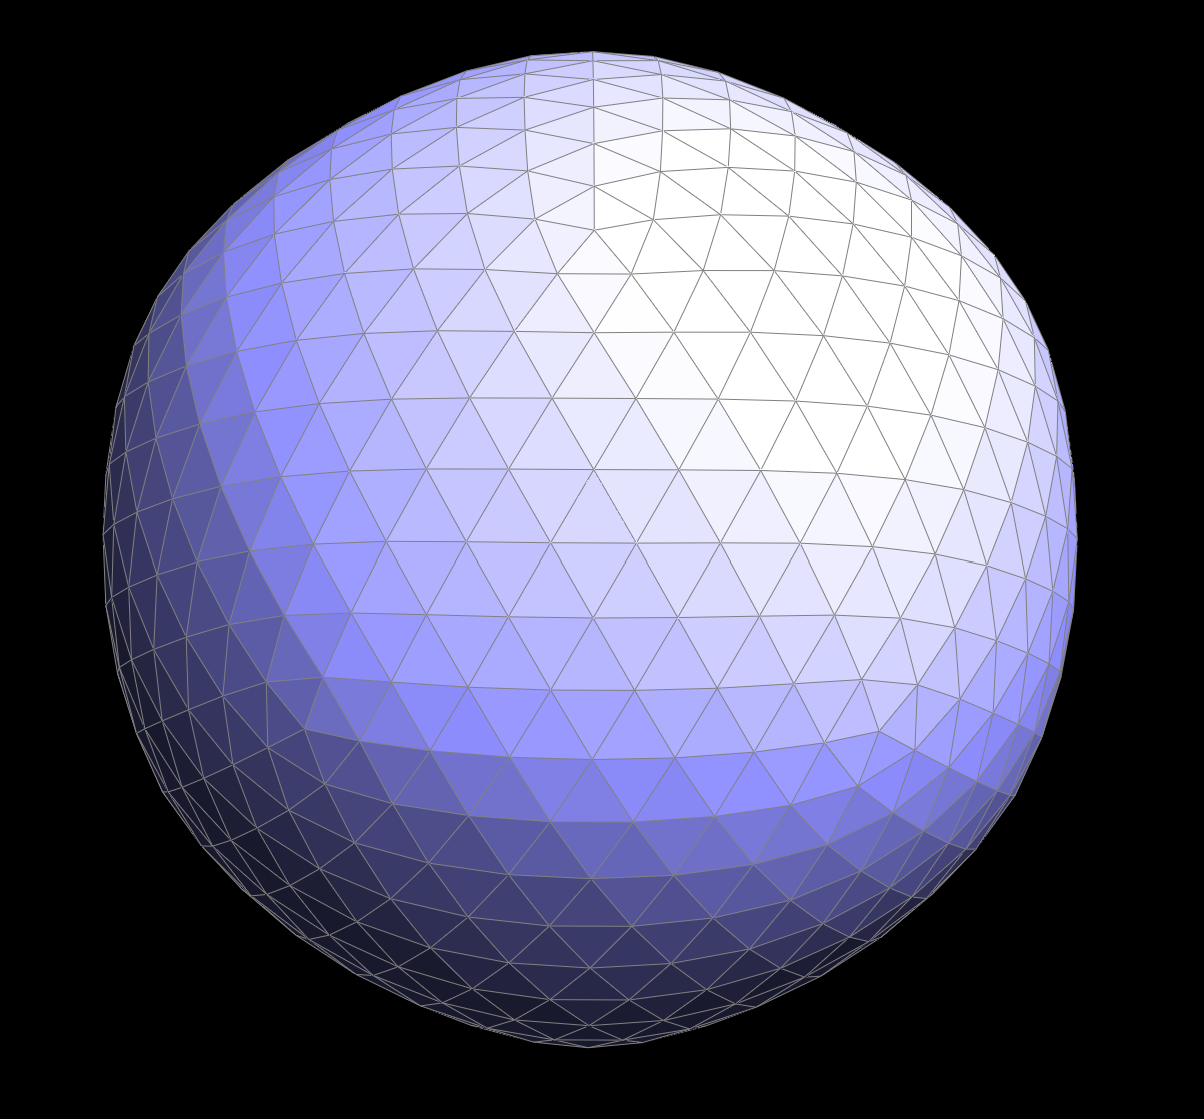
\includegraphics[]{task 6/iso4.png}
    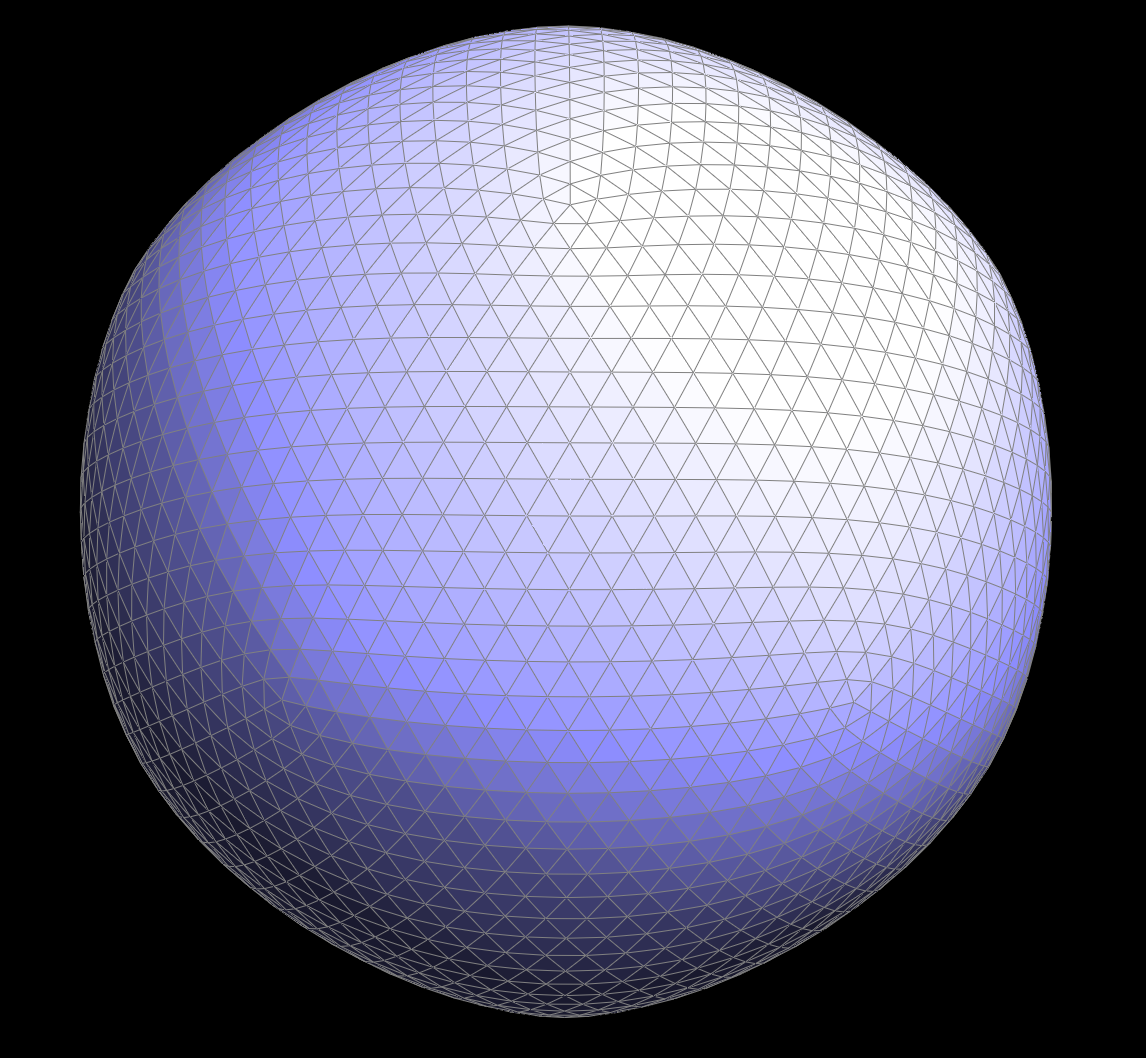
\includegraphics[]{task 6/iso5.png}
    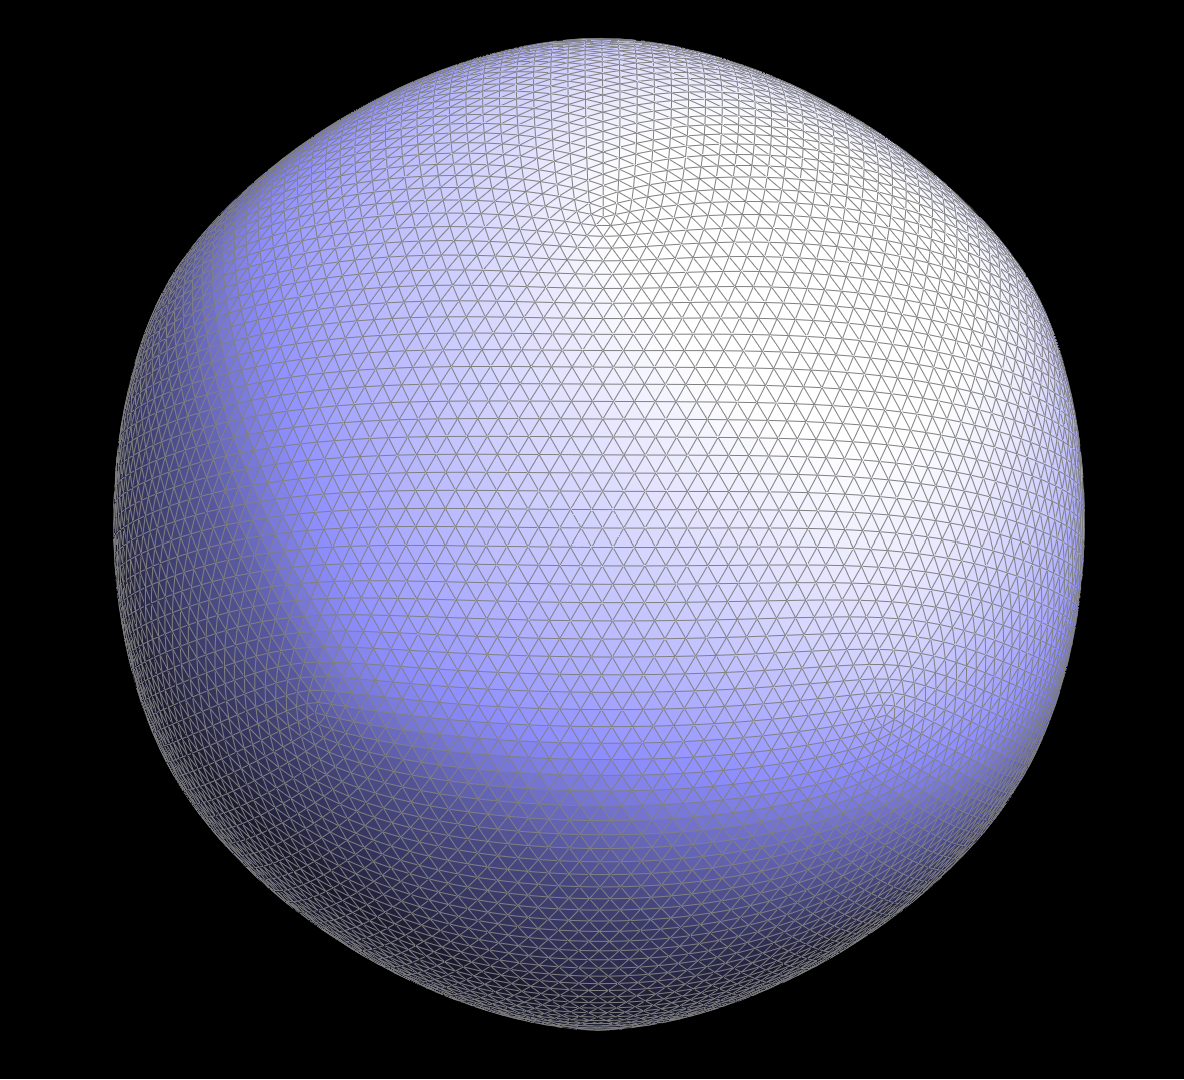
\includegraphics[]{task 6/iso6.png}
    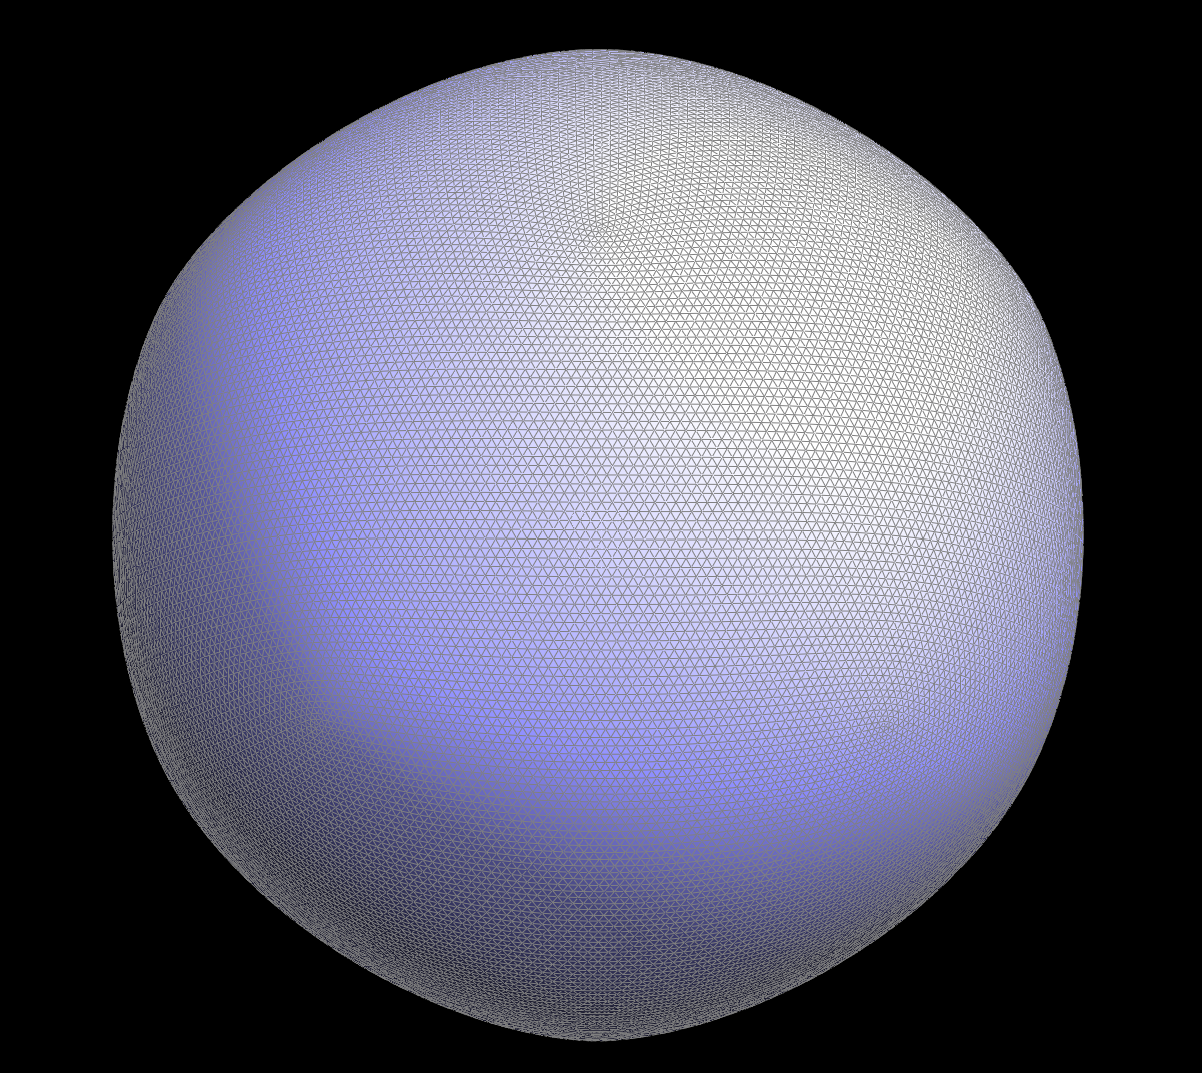
\includegraphics[]{task 6/iso7.png}
    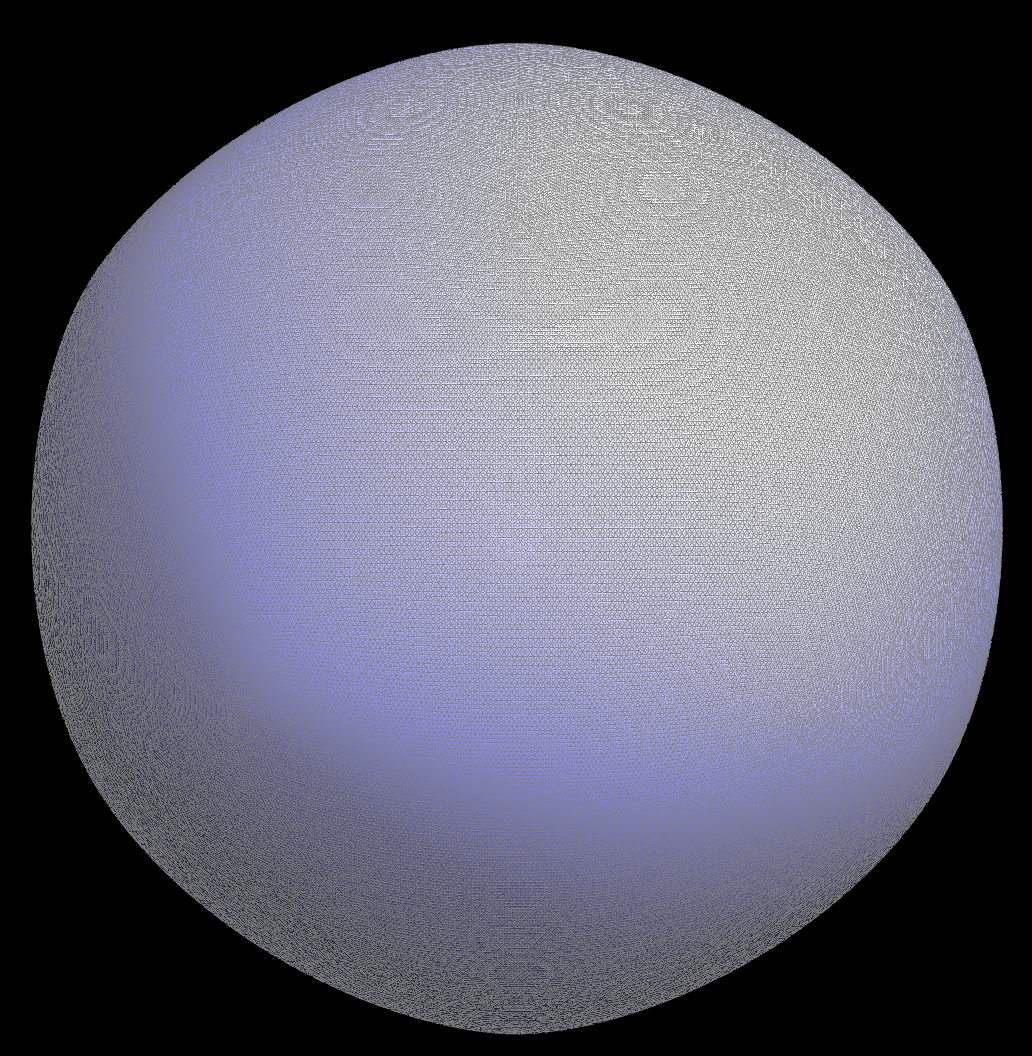
\includegraphics[]{task 6/iso8.png}
\end{center}
We can see that the icosahedron has sharp edges. However, as we keep upsampling, the sharp corners are continiously smoothened untill its a ball. To keep some of the sharpness, we can do some presplitting on the sharp edges, specifically in this fashion:
\begin{center}
    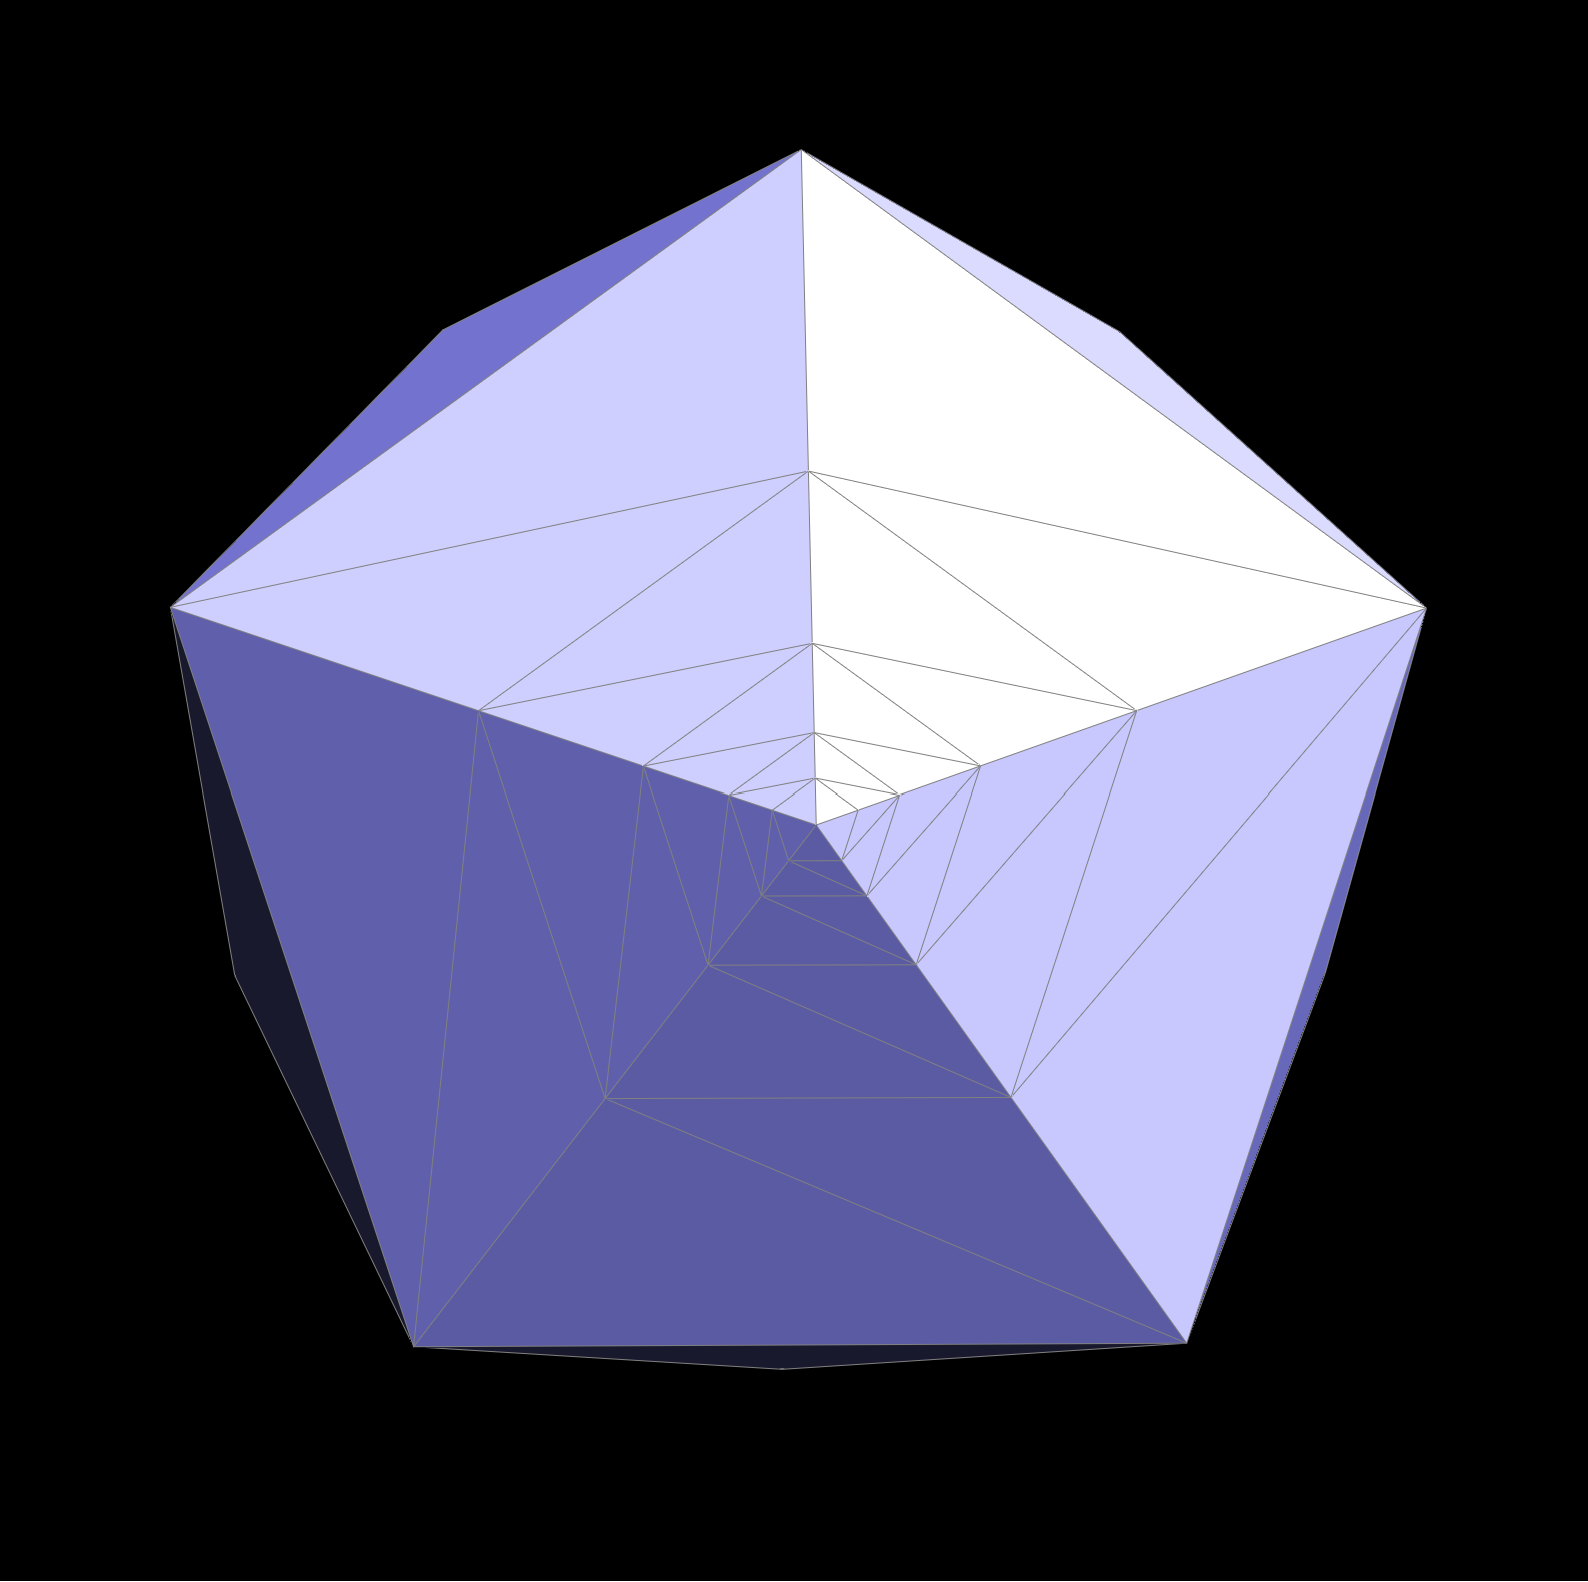
\includegraphics[]{task 6/sharp.png}
\end{center}
upsampling it gives us, looking at the side view:
\begin{center}
    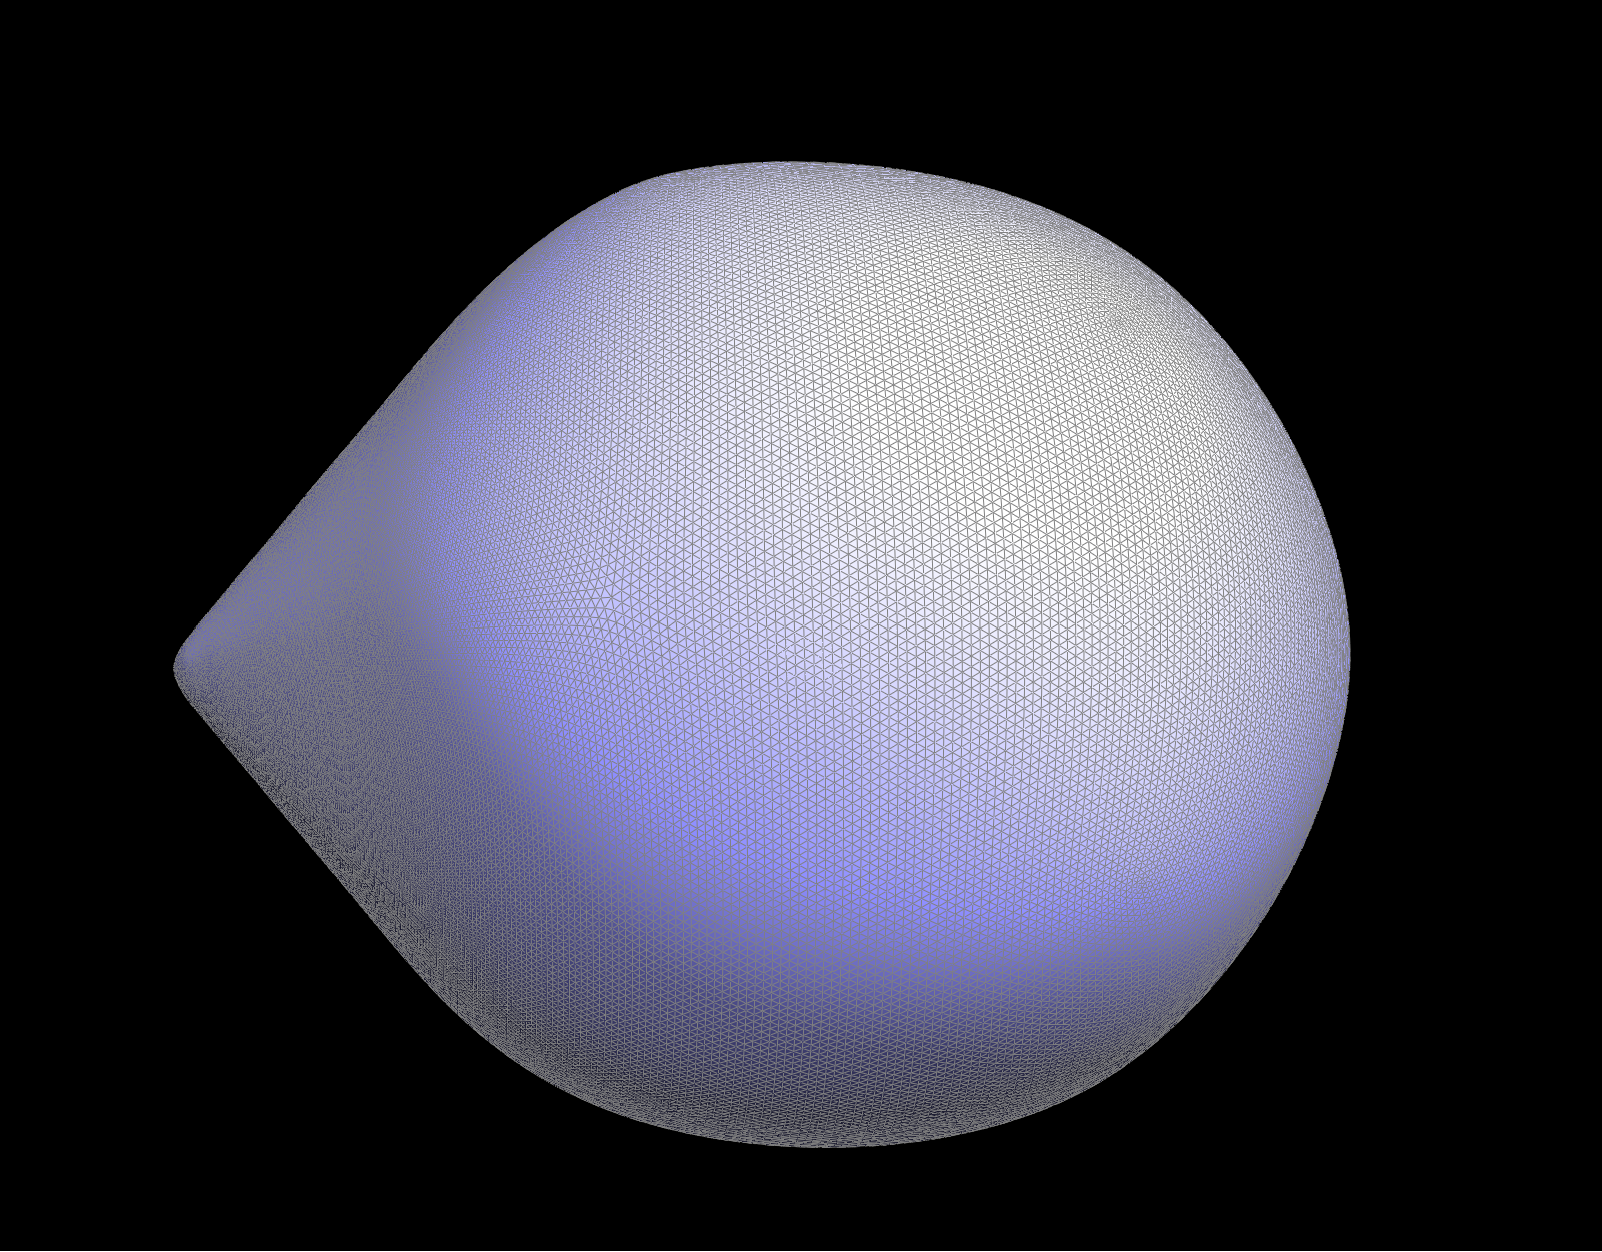
\includegraphics[]{task 6/sharpround.png}
\end{center}
This is because with more triangles, the averaging is much more accurate with the smoothing. With little triangles, the average is less accurate, so the triangles will become more concave.
\\
\\
Upsampling the cube gives us:
\begin{center}
    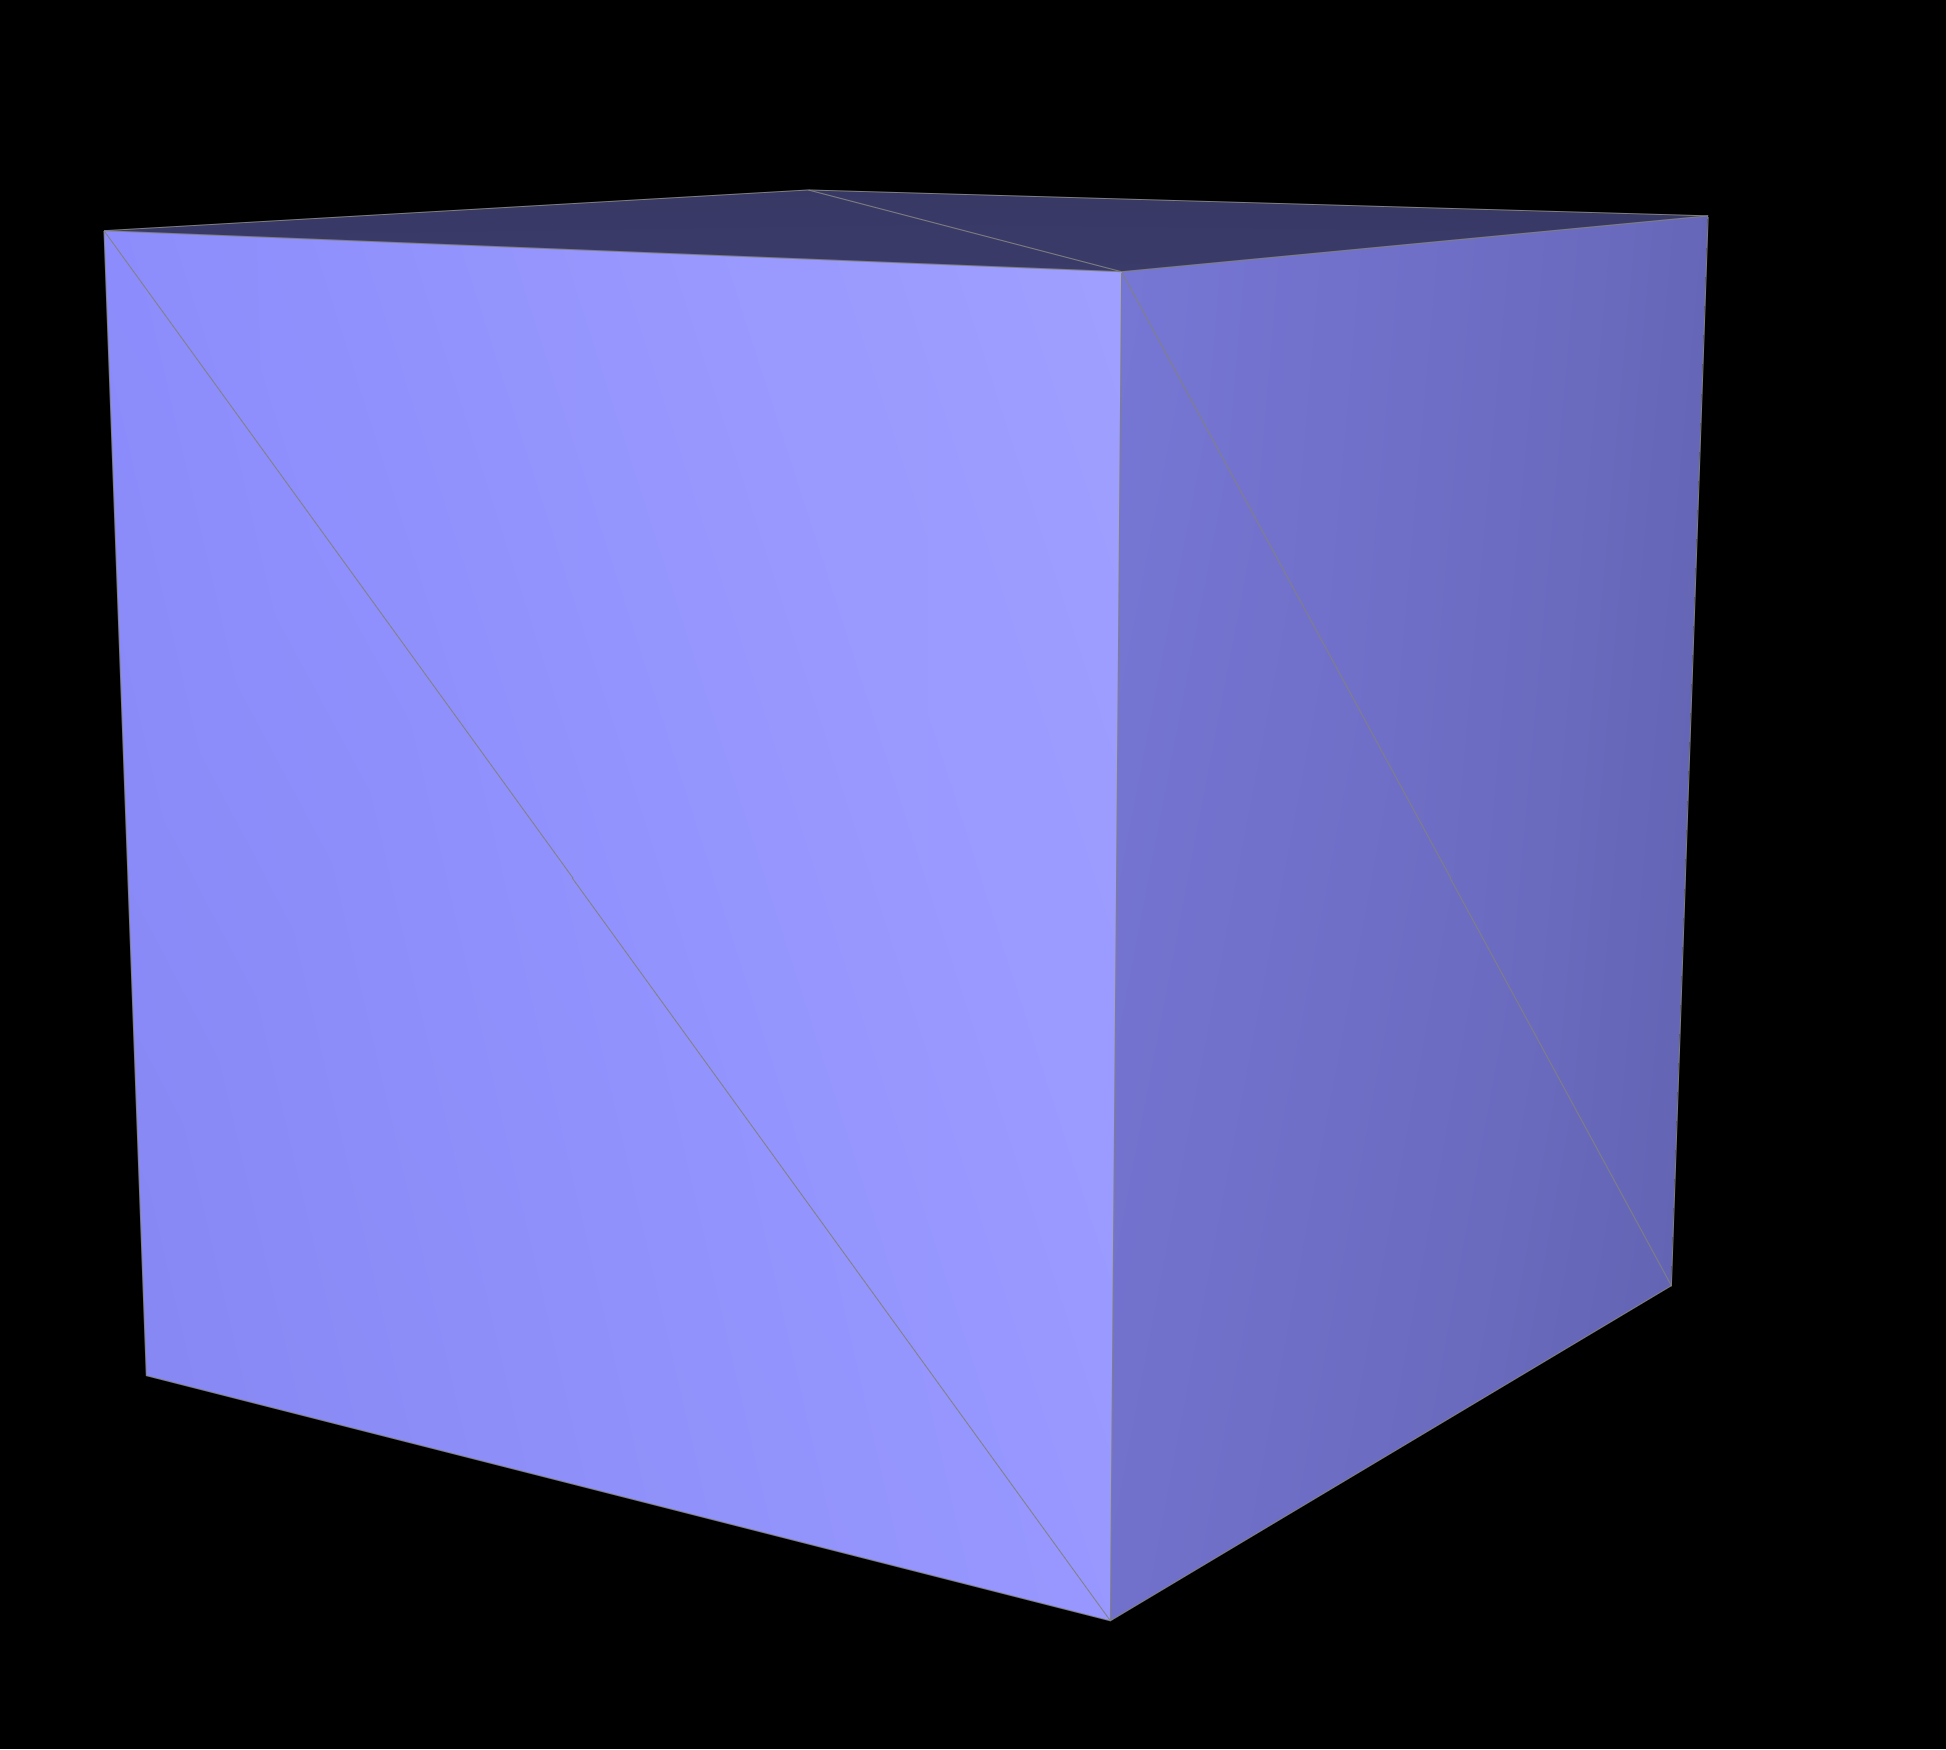
\includegraphics[]{task 6/cube1.png}
    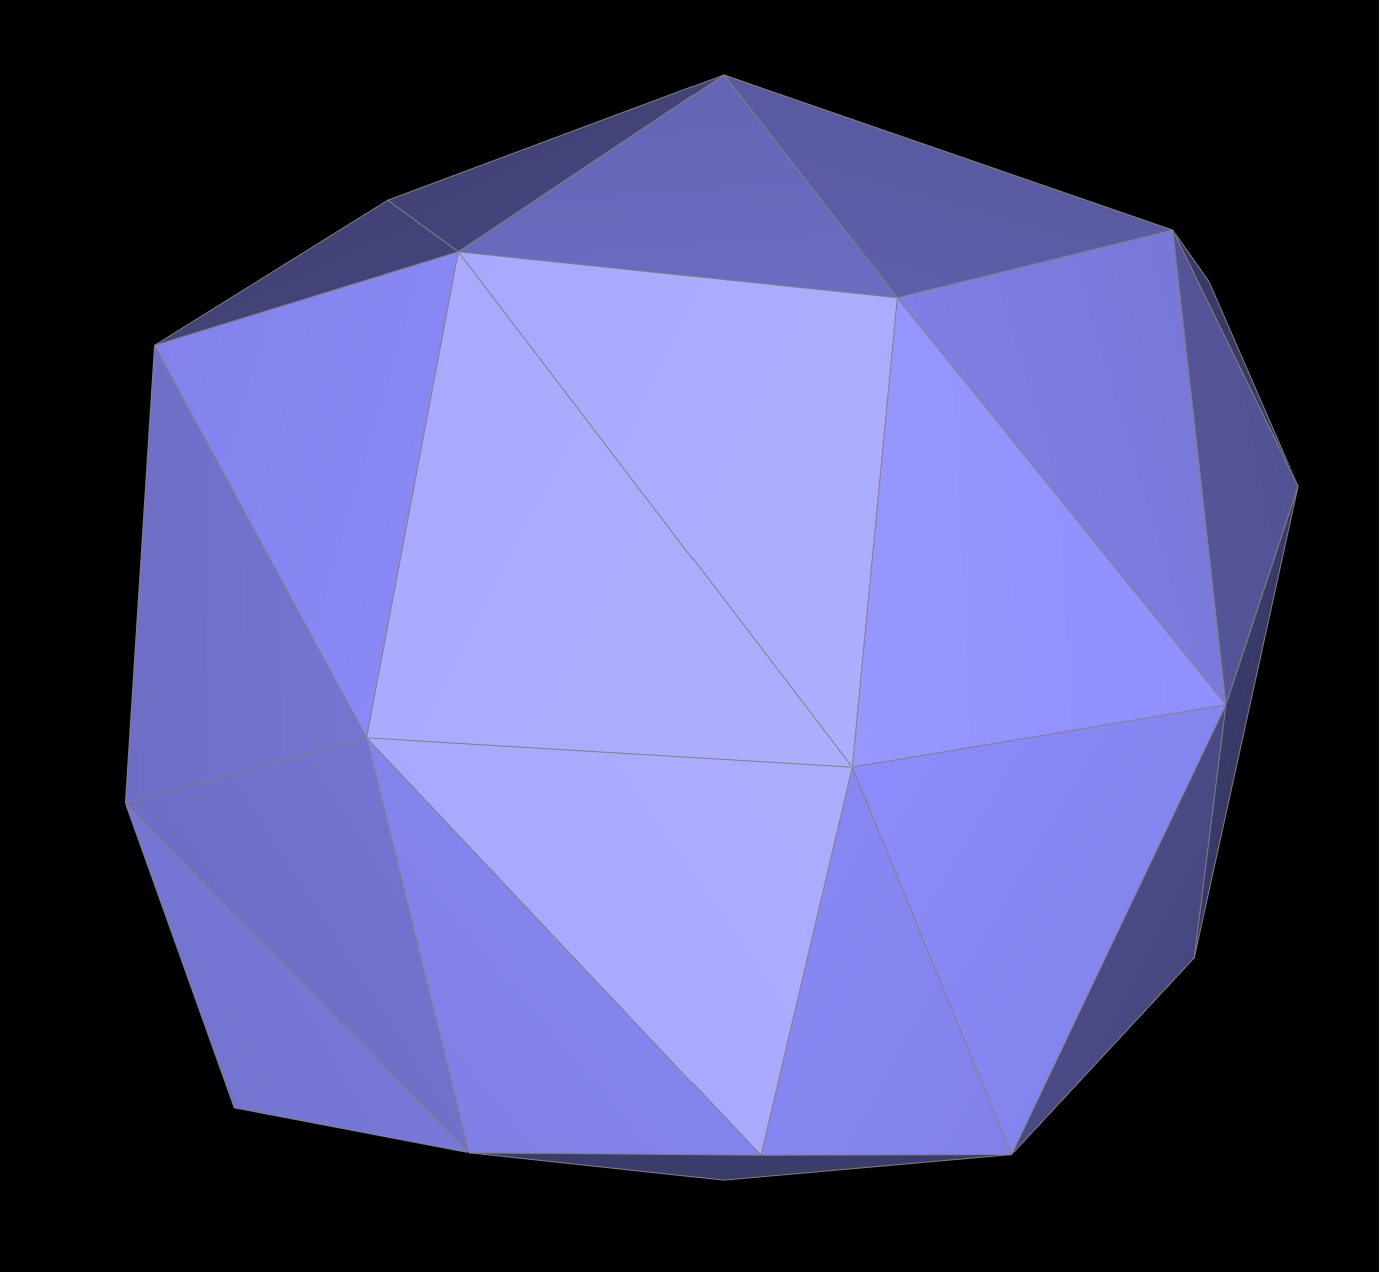
\includegraphics[]{task 6/cube2.png}

    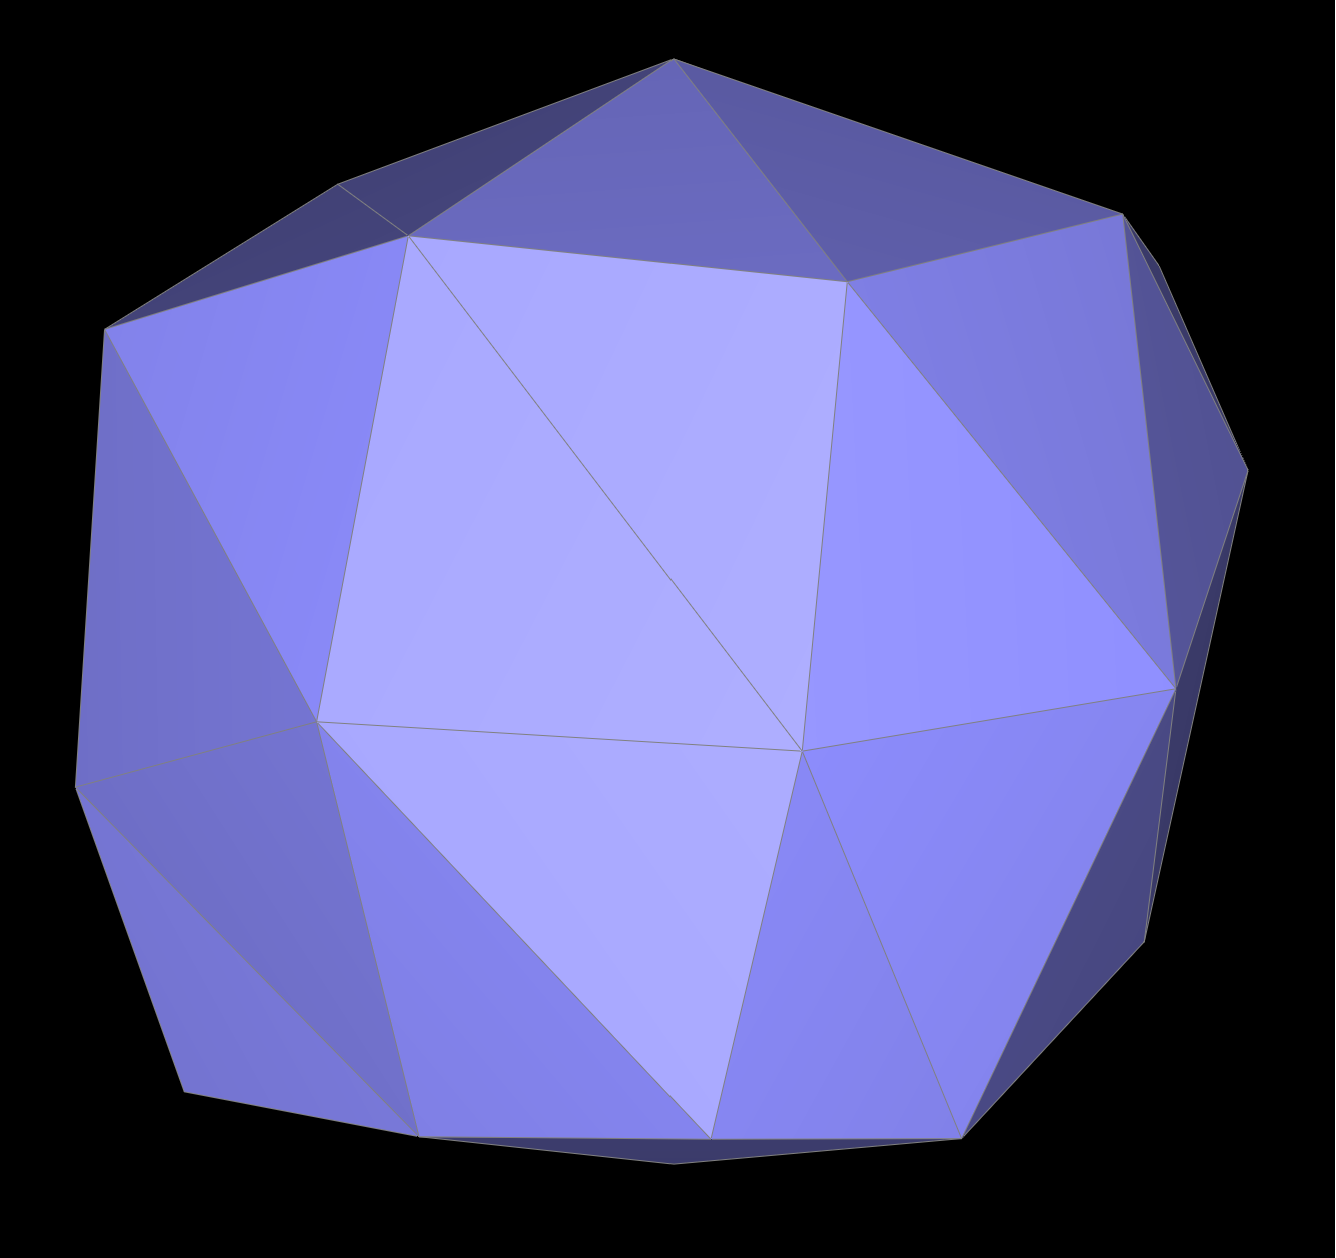
\includegraphics[]{task 6/cube3.png}

    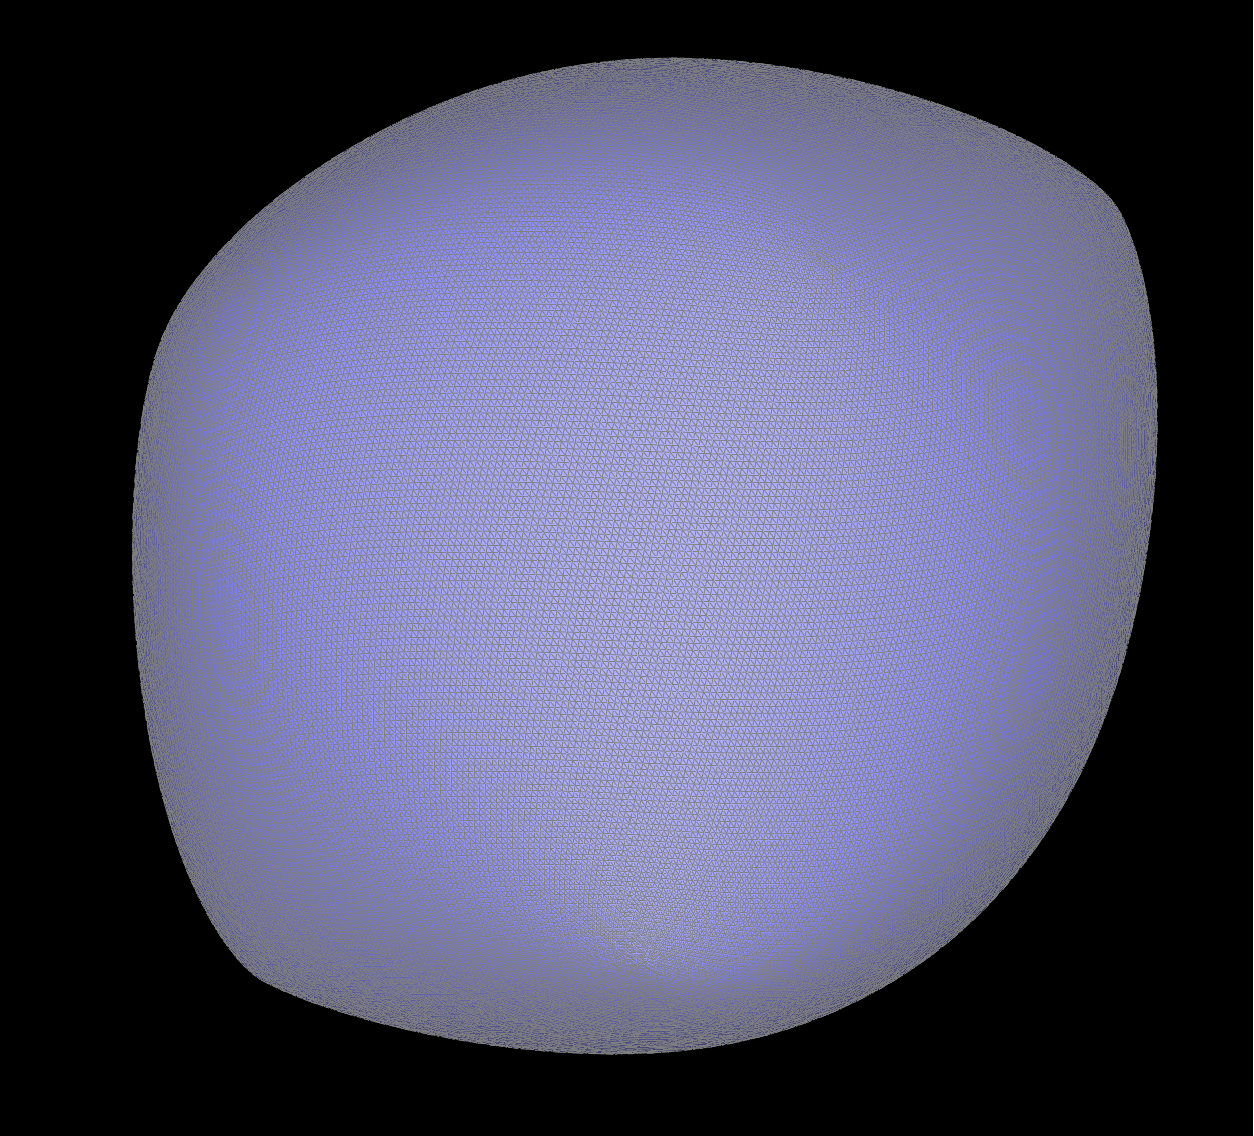
\includegraphics[]{task 6/cubeend.png}
\end{center}
We can see that the cube is upsampling unevenly. This is because the original cube triangles are assymetrical. The triangles are set up differently on different sides of the cube. To fix this, split every edge on each side of the cube so that faces are symmetrical:
\begin{center}
    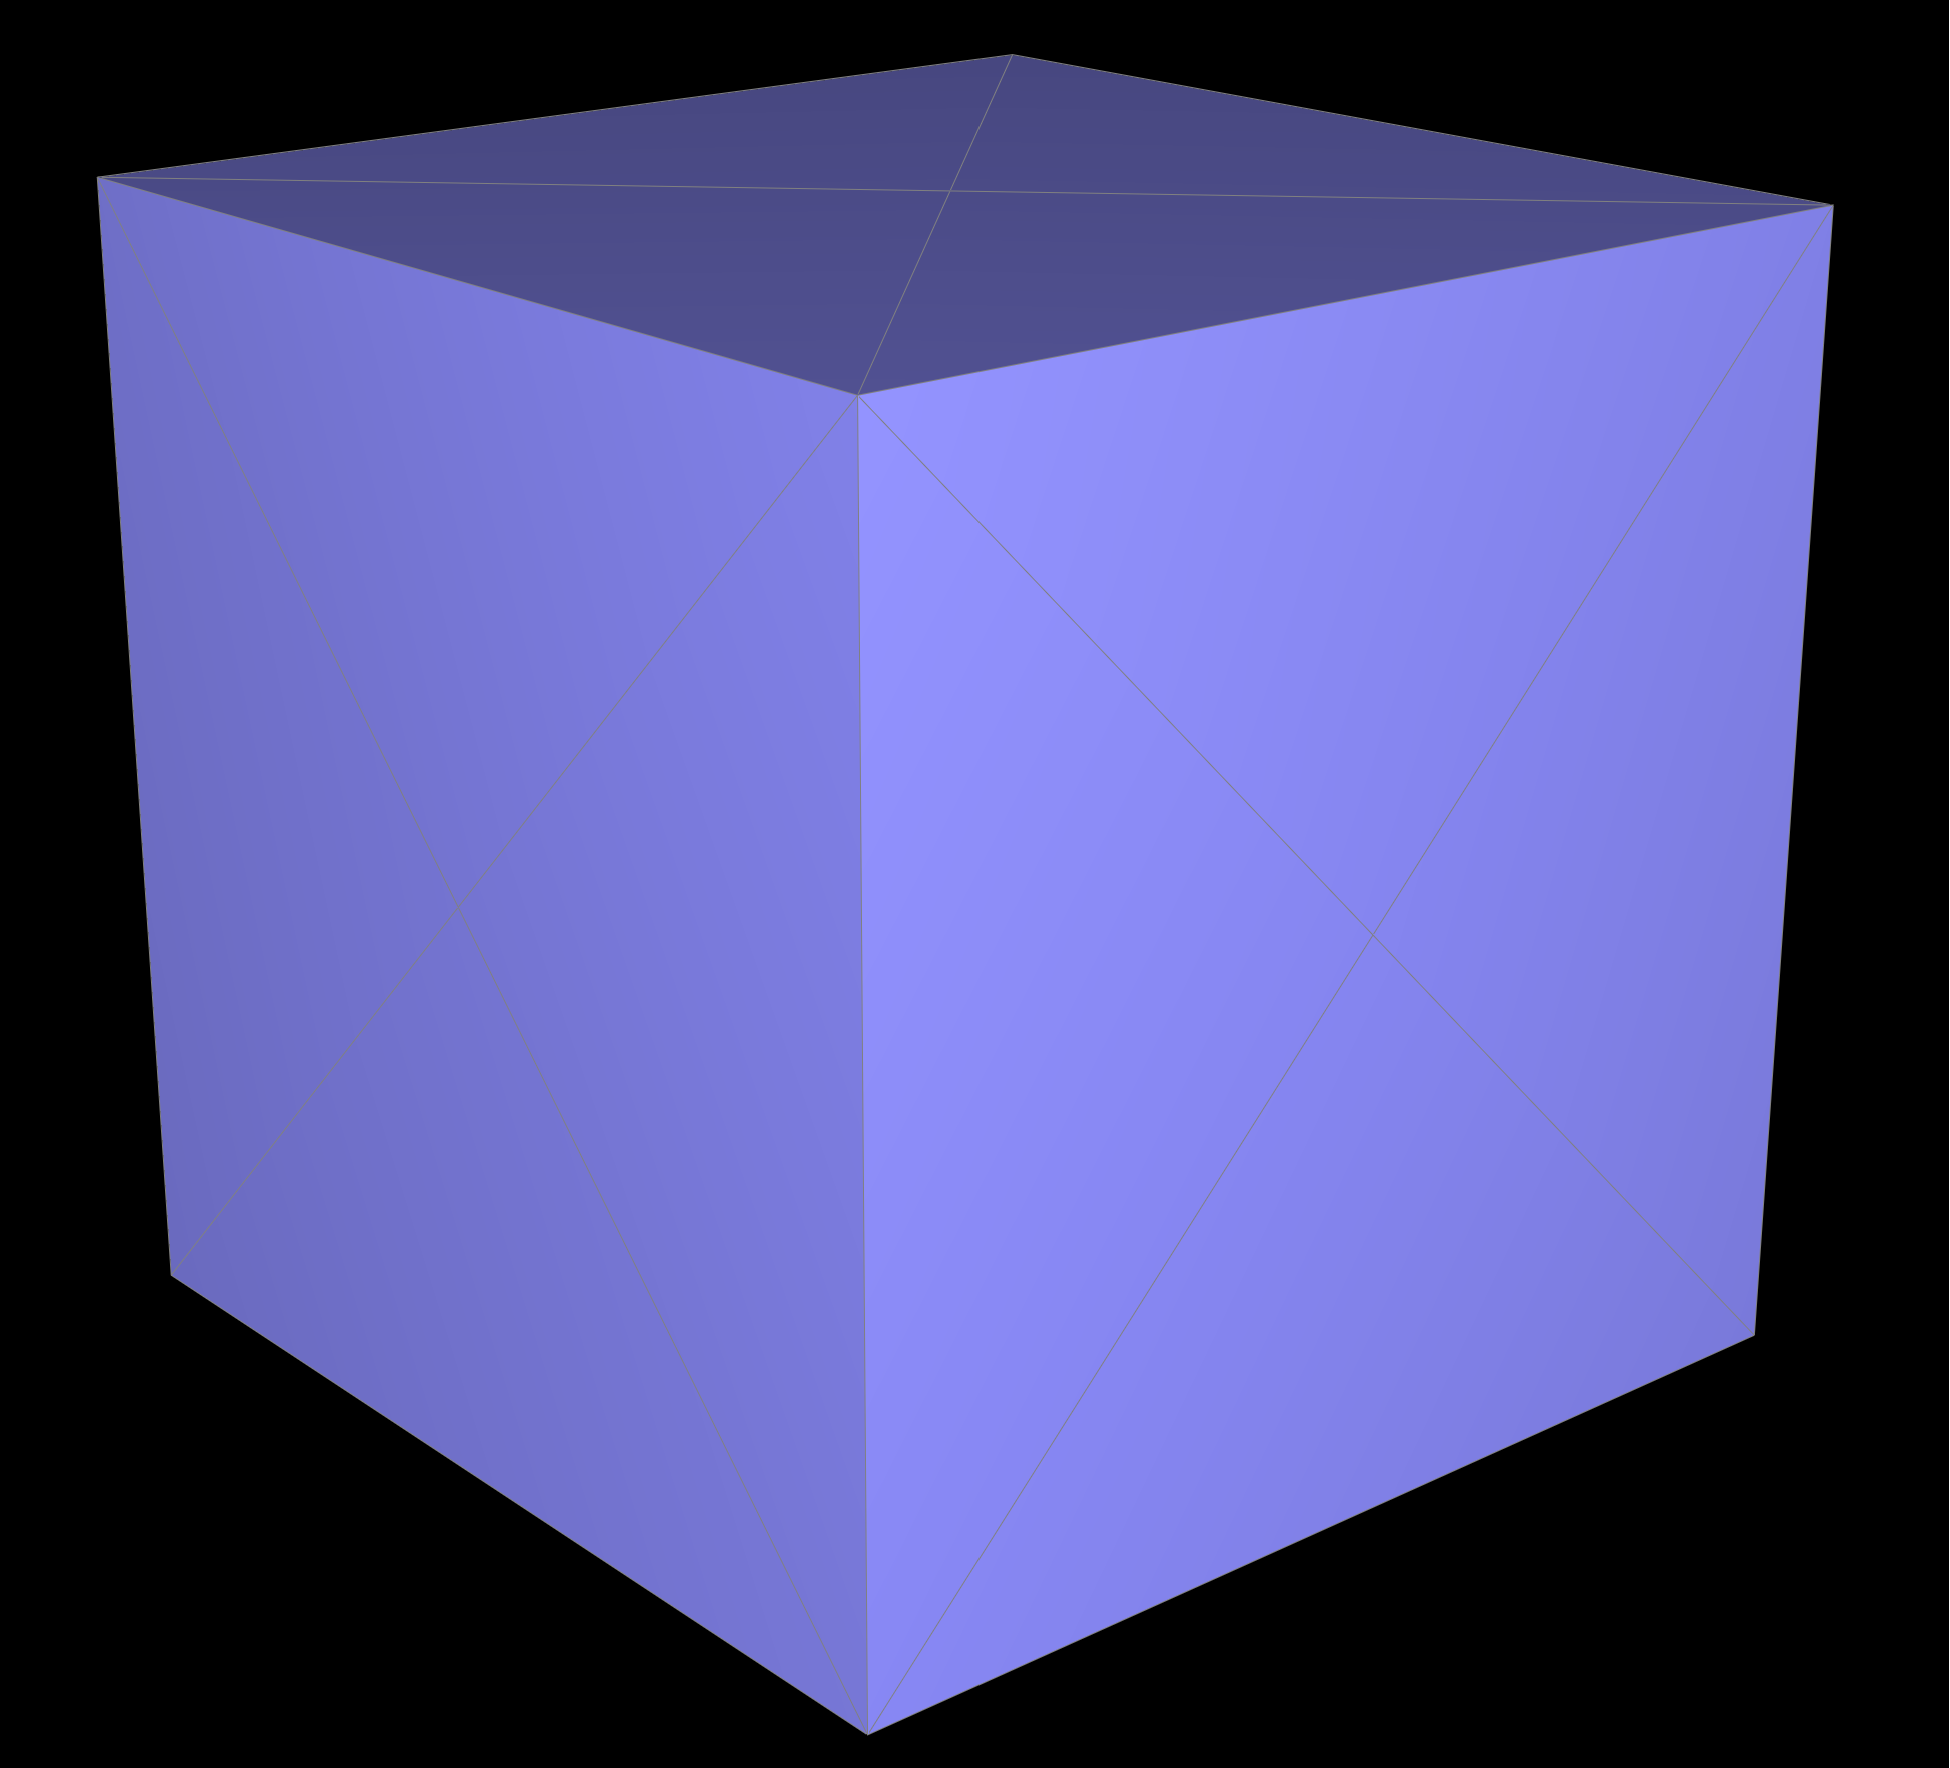
\includegraphics[]{task 6/symcube.png}

    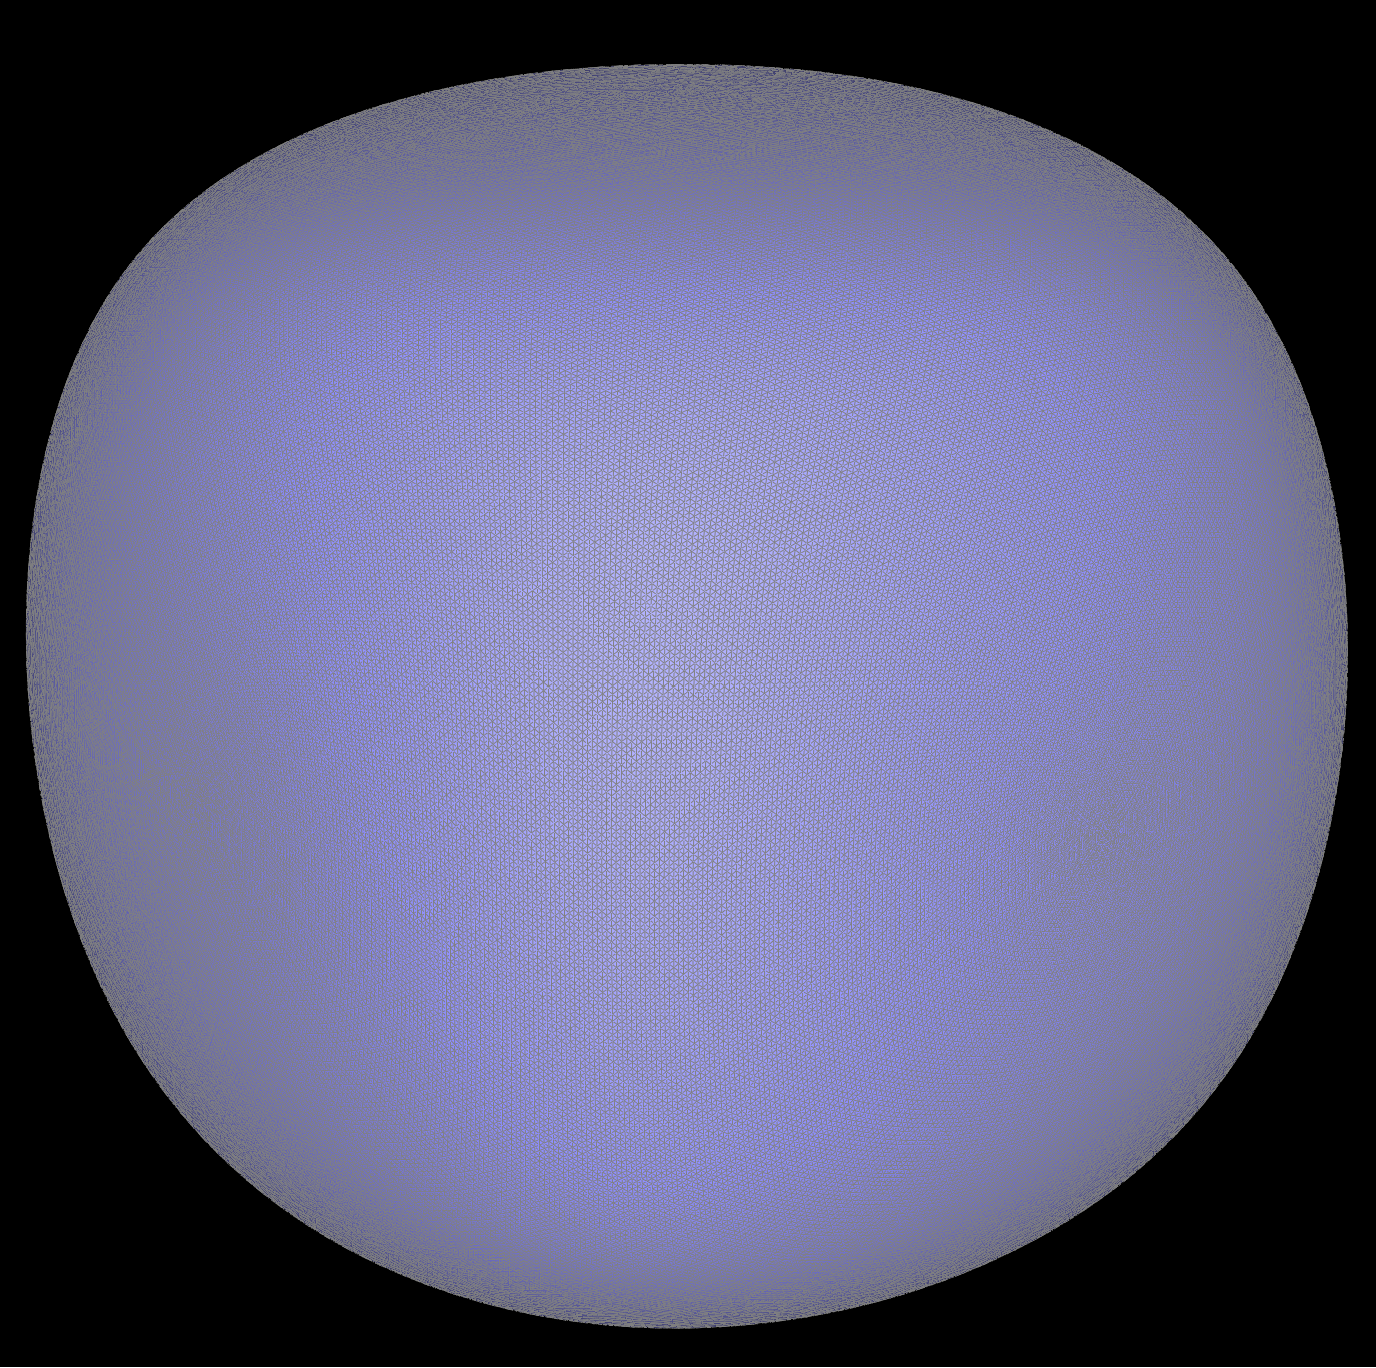
\includegraphics[]{task 6/symcubeend.png}
\end{center}
This preprocessing allows for all triangles to be upsampled symmetrically, allowing for a symmetric shape.
\end{document}
